%%%%%%%% ICML 2025 EXAMPLE LATEX SUBMISSION FILE %%%%%%%%%%%%%%%%%

\documentclass{article}
\usepackage[T1]{fontenc}
\usepackage{inconsolata}

\usepackage{enumitem}
\usepackage{hyperref}


% Attempt to make hyperref and algorithmic work together better:
\newcommand{\theHalgorithm}{\arabic{algorithm}}

% Use the following line for the initial blind version submitted for review:
\usepackage{icml2025_anon} %% DON'T USE FOR FINAL PAPER

% If accepted, instead use the following line for the camera-ready submission:
% \usepackage[accepted]{icml2025}

% For theorems and such
\newcommand{\xhdr}[1]{{\noindent\bfseries #1}.}

\usepackage{amsmath}
\usepackage{amssymb}
\usepackage{mathtools}
\usepackage{amsthm}
\usepackage{graphicx}
\usepackage{booktabs}
\usepackage{colortbl}
\usepackage{makecell}
\usepackage{caption}
\usepackage{multirow}
\usepackage{listings}
\usepackage{cuted}
\usepackage{multicol}
\usepackage{titling}
\usepackage{manyfoot}
\usepackage{verbatim}
\usepackage{xspace}
\usepackage{marginnote}
\usepackage{xcolor}
% if you use cleveref..
\usepackage[capitalize,noabbrev]{cleveref}

\usepackage{tikz}
\newcommand*\circled[1]{\tikz[baseline=(char.base)]{
            \node[shape=circle,draw,inner sep=0.5pt] (char) {#1};}}

%%%%%%%%%%%%%%%%%%%%%%%%%%%%%%%%
% THEOREMS
%%%%%%%%%%%%%%%%%%%%%%%%%%%%%%%%
\theoremstyle{plain}
\newtheorem{theorem}{Theorem}[section]
\newtheorem{proposition}[theorem]{Proposition}
\newtheorem{lemma}[theorem]{Lemma}
\newtheorem{corollary}[theorem]{Corollary}
\theoremstyle{definition}
\newtheorem{definition}[theorem]{Definition}
\newtheorem{assumption}[theorem]{Assumption}
\theoremstyle{remark}
\newtheorem{remark}[theorem]{Remark}
\usepackage{tabularx}
\usepackage{quoting}
\newenvironment{ex}[1]
 {%
  \quoting[leftmargin=0.1cm,rightmargin=0.1cm]%
  \noindent\textcolor{blue!75}{} \itshape\ignorespaces
 }
 {\endquoting}
\newcommand{\numturker}{201}
 \newcommand{\realsatisfy}{95.9\%\xspace}
 \newcommand{\realsatisfyimprov}{17.6\%\xspace}
 \newcommand{\realtimeimprov}{10.4\%\xspace}

 
\newcommand{\taskimprov}{18.5\%\xspace}
\newcommand{\itrimprov}{46.3\%\xspace}
\newcommand{\efficiencyimprov}{13.3\%\xspace}
\newcommand{\ie}{\textit{i.e., }}
\newcommand{\eg}{\textit{e.g., }}
\newcommand{\etal}{\textit{et al.}}
\newcommand{\st}{\textit{s.t. }}
\newcommand{\etc}{\textit{etc.}}
\newcommand{\wrt}{\textit{w.r.t. }}
\newcommand{\cf}{\textit{cf. }}
\newcommand{\aka}{\textit{aka. }}

% Customize monospaced font here. zi4 looks professional.
\renewcommand{\ttdefault}{zi4}

%\newcommand{\mathc }{\texttt{MATH-Chat} } 
%\newcommand{\mathct}{\texttt{MATH-Chat}} 
%\newcommand{\ambcoqa }{\texttt{Abg-CoQA} } 
%\newcommand{\ambcoqat}{\texttt{Abg-CoQa}} 
%\newcommand{\code }{\texttt{BigCodeBench-Chat} } 
%\newcommand{\codet}{\texttt{BigCodeBench-Chat}} 
%\newcommand{\doc }{\texttt{MediumDocEdit-Chat} } 
%\newcommand{\doct}{\texttt{MediumDocEdit-Chat}} 
%\newcommand{\llama}{\texttt{Meta-Llama-3.1-8B-Instruct }}
%\newcommand{\ourst}{\textsc{MR}} 
%\newcommand{\ours}{\textsc{MR }}
%\newcommand{\objectt}{interactive LLM}
%\newcommand{\object}{interactive LLM }
%\newcommand{\Objectt}{Interactive LLM}
%\newcommand{\Object}{Interactive LLM }
%\newcommand{\Objectst}{Interactive LLMs}
%\newcommand{\Objects}{Interactive LLMs }
%\newcommand{\objectst}{interactive LLMs}
%\newcommand{\objects}{interactive LLMs }

\renewcommand{\thefootnote}{\fnsymbol{footnote}}
% Please check this works, but \xspace should solve the spacing issues (the t versions could be removed).
\newcommand{\mathc}{\texttt{MATH-Chat}\xspace} 
\newcommand{\mathct}{\texttt{MATH-Chat}\xspace} 
\newcommand{\ambcoqa}{\texttt{Abg-CoQA}\xspace} 
\newcommand{\ambcoqat}{\texttt{Abg-CoQa}\xspace} 
\newcommand{\code}{\texttt{BigCodeBench-Chat}\xspace} 
\newcommand{\codet}{\texttt{BigCodeBench-Chat}\xspace} 
\newcommand{\doc}{\texttt{MediumDocEdit-Chat}\xspace} 
\newcommand{\doct}{\texttt{MediumDocEdit-Chat}\xspace} 
\newcommand{\llama}{Llama-3.1-8B\xspace}
\newcommand{\ourst}{\textsc{MR}\xspace} 
\newcommand{\ours}{\textsc{MR}\xspace}
% \newcommand{\objectt}{interactive LLM\xspace}
% \newcommand{\object}{interactive LLM\xspace}
% \newcommand{\Objectt}{Interactive LLM\xspace}
% \newcommand{\Object}{Interactive LLM\xspace}
% \newcommand{\Objectst}{Interactive LLMs\xspace}
% \newcommand{\Objects}{Interactive LLMs\xspace}
% \newcommand{\objectst}{interactive LLMs\xspace}
% \newcommand{\objects}{interactive LLMs\xspace}

\newcommand{\name}{\textsc{CollabLLM}\xspace}
\newcommand{\namewithspace}{\textsc{Collab LLM}\xspace}
\newcommand{\objectt}{collaborative LLM\xspace}
\newcommand{\object}{collaborative LLM\xspace}
\newcommand{\Objectt}{Collaborative LLM\xspace}
\newcommand{\Object}{Collaborative LLM\xspace}
\newcommand{\Objectst}{Collaborative LLMs\xspace}
\newcommand{\Objects}{Collaborative LLMs\xspace}
\newcommand{\objectst}{collaborative LLMs\xspace}
\newcommand{\objects}{collaborative LLMs\xspace}
\usepackage{inconsolata} % Import modern font package
\lstset{
  basicstyle=\fontfamily{pcr}\selectfont\itshape\small, % Monospace + Italic + Small font
  frame=tb,                   
  breaklines=true,             
  breakatwhitespace=false,     
  linewidth=\linewidth,        
  numbers=left,                
  numberstyle=\tiny\color{gray}, 
  xleftmargin=10pt,            
  framexleftmargin=10pt,       
  tabsize=4,                   
  showstringspaces=false,      
  keywordstyle=\color{blue}\bfseries,  
  commentstyle=\color{gray},   
  stringstyle=\color{red},     
  aboveskip=10pt,              
  belowskip=10pt               
}
\usepackage{pifont}
\usepackage{xcolor}
% Changes globally:
\setlist[itemize]{leftmargin=10pt, itemsep=0pt, topsep=0pt, parsep=0pt}

%\newcommand{\TODO}[2]{\textcolor{red}{\textbf{TODO (#1)}: \textit{#2}}}
%\newcommand{\jure}[1]{\textcolor{red}{\textbf{Jure}: \textit{#1}}}
%\newcommand{\james}[1]{\textcolor{blue}{\textbf{James}: \textit{#1}}}
% \newcommand{\jure}[1]{\marginnote{\textcolor{red}{\textbf{Jure}: \textit{#1}}}}
% \newcommand{\james}[1]{\marginnote{\textcolor{blue}{\textbf{James}: \textit{#1}}}}

% Todonotes is useful during development; simply uncomment the next line
%    and comment out the line below the next line to turn off comments
%\usepackage[disable,textsize=tiny]{todonotes}
\usepackage[textsize=tiny]{todonotes}


% The \icmltitle you define below is probably too long as a header.
% Therefore, a short form for the running title is supplied here:
\icmltitlerunning{\name{}: From Passive Responders to Active Collaborators}

\begin{document}
\onecolumn  % Hank Hack
% \twocolumn[  % Hank Hack
\icmltitle{\name{}: From Passive Responders to Active Collaborators}

% It is OKAY to include author information, even for blind
% submissions: the style file will automatically remove it for you
% unless you've provided the [accepted] option to the icml2025
% package.

% List of affiliations: The first argument should be a (short)
% identifier you will use later to specify author affiliations
% Academic affiliations should list Department, University, City, Region, Country
% Industry affiliations should list Company, City, Region, Country

% You can specify symbols, otherwise they are numbered in order.
% Ideally, you should not use this facility. Affiliations will be numbered
% in order of appearance and this is the preferred way.
% \icmlsetsymbol{equal}{*}

\begin{icmlauthorlist}
\icmlauthor{Firstname1 Lastname1}{equal,yyy}
\icmlauthor{Firstname2 Lastname2}{equal,yyy,comp}
\end{icmlauthorlist}

% \author{Shirley Wu$^1$\thanks{Major work done at Microsoft Research. Correspondence: \{shirwu@cs.stanford.edu, mgalley@microsoft.com\}}\ ,\ Michel Galley$^2$,\ Baolin Peng$^2$,\ Hao Cheng$^2$,\ Yao Dou$^3$, Weixin Cai$^2$,\ \\
% \textbf{Jure Leskovec}$^1$, \textbf{James Zou}$^1$,\ \textbf{Jianfeng Gao}$^2$\\
% $^1$ Stanford University\quad $^2$ Microsoft Research\\
% % (--Tentative, free to edit anything)\\
% \vspace{20pt}
% }
\icmlaffiliation{}{}
\icmlaffiliation{comp}{Company Name, Location, Country}
\icmlaffiliation{sch}{School of ZZZ, Institute of WWW, Location, Country}

\icmlcorrespondingauthor{anonymous}{anonymous}

% You may provide any keywords that you
% find helpful for describing your paper; these are used to populate
% the "keywords" metadata in the PDF but will not be shown in the document
\icmlkeywords{Machine Learning, ICML}

\vskip 0.3in
% ] 

\begin{figure}[H]
    \centering
    \vspace{-28pt}
    \includegraphics[width=0.87\linewidth]{figures/cropped/first_v7b}
    %\includegraphics[width=0.87\linewidth]{figures/first_v5}
    \vspace{-5pt}
    \captionof{figure}{\name{} Framework: Given a context \circled{\small 1}, the model generates a response \circled{\small 2} to maximize long-term collaboration gains, termed \textit{Multiturn-aware Rewards} (MR). During training, MRs are estimated via \circled{\small 3} collaborative simulation, which forward-samples conversations with simulated users.
    %and computes averaged conversation-level rewards. 
    Finally, \circled{\small 4} reinforcement fine-tuning is applied using the MRs.
    %OLD: \captionof{figure}{\name{} Training Framework: Given a context \circled{\small 1}, the model aims to generate a response \circled{\small 2} maximizing long-term collaboration gains, referred to as \textit{Multiturn-aware Rewards} (MR). During training, MRs are estimated through \circled{\small 3} collaborative simulation, which involves forward sampling to generate future conversations with simulated users and computing the average conversation-level reward. Finally, \circled{\small 4} reinforcement fine-tuning is performed using the MRs.
    }
     % by \eg suggesting follow-up questions or alternative explorations. 
    %\captionof{figure}{Our interactive LLM training framework: Given a context, our models learn to maximize long-term gains, encouraging the model to effectively collaborate with real users, \eg by proposing follow-up questions or alternative explorations.}
    %\captionof{figure}{Our interactive LLM training framework. Given a context, our framework trains the LLM to output responses that maximize long-term gains instead of intermediate rewards, encouraging the model to effectively collaborate with real users, \eg by proposing follow-up questions or alternative explorations.}
    \label{fig:overview}
\end{figure}

\begin{multicols}{2}  % Hank Hack
% this must go after the closing bracket ] following \twocolumn[ ...

% This command actually creates the footnote in the first column
% listing the affiliations and the copyright notice.
% The command takes one argument, which is text to display at the start of the footnote.
% The \icmlEqualContribution command is standard text for equal contribution.
% Remove it (just {}) if you do not need this facility.

%\printAffiliationsAndNotice{}  % leave blank if no need to mention equal contribution
\printAffiliationsAndNotice{} % otherwise use the standard text.


\begin{abstract}  
Test time scaling is currently one of the most active research areas that shows promise after training time scaling has reached its limits.
Deep-thinking (DT) models are a class of recurrent models that can perform easy-to-hard generalization by assigning more compute to harder test samples.
However, due to their inability to determine the complexity of a test sample, DT models have to use a large amount of computation for both easy and hard test samples.
Excessive test time computation is wasteful and can cause the ``overthinking'' problem where more test time computation leads to worse results.
In this paper, we introduce a test time training method for determining the optimal amount of computation needed for each sample during test time.
We also propose Conv-LiGRU, a novel recurrent architecture for efficient and robust visual reasoning. 
Extensive experiments demonstrate that Conv-LiGRU is more stable than DT, effectively mitigates the ``overthinking'' phenomenon, and achieves superior accuracy.
\end{abstract}  
\section{Introduction}
\label{sec:introduction}
The business processes of organizations are experiencing ever-increasing complexity due to the large amount of data, high number of users, and high-tech devices involved \cite{martin2021pmopportunitieschallenges, beerepoot2023biggestbpmproblems}. This complexity may cause business processes to deviate from normal control flow due to unforeseen and disruptive anomalies \cite{adams2023proceddsriftdetection}. These control-flow anomalies manifest as unknown, skipped, and wrongly-ordered activities in the traces of event logs monitored from the execution of business processes \cite{ko2023adsystematicreview}. For the sake of clarity, let us consider an illustrative example of such anomalies. Figure \ref{FP_ANOMALIES} shows a so-called event log footprint, which captures the control flow relations of four activities of a hypothetical event log. In particular, this footprint captures the control-flow relations between activities \texttt{a}, \texttt{b}, \texttt{c} and \texttt{d}. These are the causal ($\rightarrow$) relation, concurrent ($\parallel$) relation, and other ($\#$) relations such as exclusivity or non-local dependency \cite{aalst2022pmhandbook}. In addition, on the right are six traces, of which five exhibit skipped, wrongly-ordered and unknown control-flow anomalies. For example, $\langle$\texttt{a b d}$\rangle$ has a skipped activity, which is \texttt{c}. Because of this skipped activity, the control-flow relation \texttt{b}$\,\#\,$\texttt{d} is violated, since \texttt{d} directly follows \texttt{b} in the anomalous trace.
\begin{figure}[!t]
\centering
\includegraphics[width=0.9\columnwidth]{images/FP_ANOMALIES.png}
\caption{An example event log footprint with six traces, of which five exhibit control-flow anomalies.}
\label{FP_ANOMALIES}
\end{figure}

\subsection{Control-flow anomaly detection}
Control-flow anomaly detection techniques aim to characterize the normal control flow from event logs and verify whether these deviations occur in new event logs \cite{ko2023adsystematicreview}. To develop control-flow anomaly detection techniques, \revision{process mining} has seen widespread adoption owing to process discovery and \revision{conformance checking}. On the one hand, process discovery is a set of algorithms that encode control-flow relations as a set of model elements and constraints according to a given modeling formalism \cite{aalst2022pmhandbook}; hereafter, we refer to the Petri net, a widespread modeling formalism. On the other hand, \revision{conformance checking} is an explainable set of algorithms that allows linking any deviations with the reference Petri net and providing the fitness measure, namely a measure of how much the Petri net fits the new event log \cite{aalst2022pmhandbook}. Many control-flow anomaly detection techniques based on \revision{conformance checking} (hereafter, \revision{conformance checking}-based techniques) use the fitness measure to determine whether an event log is anomalous \cite{bezerra2009pmad, bezerra2013adlogspais, myers2018icsadpm, pecchia2020applicationfailuresanalysispm}. 

The scientific literature also includes many \revision{conformance checking}-independent techniques for control-flow anomaly detection that combine specific types of trace encodings with machine/deep learning \cite{ko2023adsystematicreview, tavares2023pmtraceencoding}. Whereas these techniques are very effective, their explainability is challenging due to both the type of trace encoding employed and the machine/deep learning model used \cite{rawal2022trustworthyaiadvances,li2023explainablead}. Hence, in the following, we focus on the shortcomings of \revision{conformance checking}-based techniques to investigate whether it is possible to support the development of competitive control-flow anomaly detection techniques while maintaining the explainable nature of \revision{conformance checking}.
\begin{figure}[!t]
\centering
\includegraphics[width=\columnwidth]{images/HIGH_LEVEL_VIEW.png}
\caption{A high-level view of the proposed framework for combining \revision{process mining}-based feature extraction with dimensionality reduction for control-flow anomaly detection.}
\label{HIGH_LEVEL_VIEW}
\end{figure}

\subsection{Shortcomings of \revision{conformance checking}-based techniques}
Unfortunately, the detection effectiveness of \revision{conformance checking}-based techniques is affected by noisy data and low-quality Petri nets, which may be due to human errors in the modeling process or representational bias of process discovery algorithms \cite{bezerra2013adlogspais, pecchia2020applicationfailuresanalysispm, aalst2016pm}. Specifically, on the one hand, noisy data may introduce infrequent and deceptive control-flow relations that may result in inconsistent fitness measures, whereas, on the other hand, checking event logs against a low-quality Petri net could lead to an unreliable distribution of fitness measures. Nonetheless, such Petri nets can still be used as references to obtain insightful information for \revision{process mining}-based feature extraction, supporting the development of competitive and explainable \revision{conformance checking}-based techniques for control-flow anomaly detection despite the problems above. For example, a few works outline that token-based \revision{conformance checking} can be used for \revision{process mining}-based feature extraction to build tabular data and develop effective \revision{conformance checking}-based techniques for control-flow anomaly detection \cite{singh2022lapmsh, debenedictis2023dtadiiot}. However, to the best of our knowledge, the scientific literature lacks a structured proposal for \revision{process mining}-based feature extraction using the state-of-the-art \revision{conformance checking} variant, namely alignment-based \revision{conformance checking}.

\subsection{Contributions}
We propose a novel \revision{process mining}-based feature extraction approach with alignment-based \revision{conformance checking}. This variant aligns the deviating control flow with a reference Petri net; the resulting alignment can be inspected to extract additional statistics such as the number of times a given activity caused mismatches \cite{aalst2022pmhandbook}. We integrate this approach into a flexible and explainable framework for developing techniques for control-flow anomaly detection. The framework combines \revision{process mining}-based feature extraction and dimensionality reduction to handle high-dimensional feature sets, achieve detection effectiveness, and support explainability. Notably, in addition to our proposed \revision{process mining}-based feature extraction approach, the framework allows employing other approaches, enabling a fair comparison of multiple \revision{conformance checking}-based and \revision{conformance checking}-independent techniques for control-flow anomaly detection. Figure \ref{HIGH_LEVEL_VIEW} shows a high-level view of the framework. Business processes are monitored, and event logs obtained from the database of information systems. Subsequently, \revision{process mining}-based feature extraction is applied to these event logs and tabular data input to dimensionality reduction to identify control-flow anomalies. We apply several \revision{conformance checking}-based and \revision{conformance checking}-independent framework techniques to publicly available datasets, simulated data of a case study from railways, and real-world data of a case study from healthcare. We show that the framework techniques implementing our approach outperform the baseline \revision{conformance checking}-based techniques while maintaining the explainable nature of \revision{conformance checking}.

In summary, the contributions of this paper are as follows.
\begin{itemize}
    \item{
        A novel \revision{process mining}-based feature extraction approach to support the development of competitive and explainable \revision{conformance checking}-based techniques for control-flow anomaly detection.
    }
    \item{
        A flexible and explainable framework for developing techniques for control-flow anomaly detection using \revision{process mining}-based feature extraction and dimensionality reduction.
    }
    \item{
        Application to synthetic and real-world datasets of several \revision{conformance checking}-based and \revision{conformance checking}-independent framework techniques, evaluating their detection effectiveness and explainability.
    }
\end{itemize}

The rest of the paper is organized as follows.
\begin{itemize}
    \item Section \ref{sec:related_work} reviews the existing techniques for control-flow anomaly detection, categorizing them into \revision{conformance checking}-based and \revision{conformance checking}-independent techniques.
    \item Section \ref{sec:abccfe} provides the preliminaries of \revision{process mining} to establish the notation used throughout the paper, and delves into the details of the proposed \revision{process mining}-based feature extraction approach with alignment-based \revision{conformance checking}.
    \item Section \ref{sec:framework} describes the framework for developing \revision{conformance checking}-based and \revision{conformance checking}-independent techniques for control-flow anomaly detection that combine \revision{process mining}-based feature extraction and dimensionality reduction.
    \item Section \ref{sec:evaluation} presents the experiments conducted with multiple framework and baseline techniques using data from publicly available datasets and case studies.
    \item Section \ref{sec:conclusions} draws the conclusions and presents future work.
\end{itemize}
\section{Method}\label{sec:method}
\begin{figure}
    \centering
    \includegraphics[width=0.85\textwidth]{imgs/heatmap_acc.pdf}
    \caption{\textbf{Visualization of the proposed periodic Bayesian flow with mean parameter $\mu$ and accumulated accuracy parameter $c$ which corresponds to the entropy/uncertainty}. For $x = 0.3, \beta(1) = 1000$ and $\alpha_i$ defined in \cref{appd:bfn_cir}, this figure plots three colored stochastic parameter trajectories for receiver mean parameter $m$ and accumulated accuracy parameter $c$, superimposed on a log-scale heatmap of the Bayesian flow distribution $p_F(m|x,\senderacc)$ and $p_F(c|x,\senderacc)$. Note the \emph{non-monotonicity} and \emph{non-additive} property of $c$ which could inform the network the entropy of the mean parameter $m$ as a condition and the \emph{periodicity} of $m$. %\jj{Shrink the figures to save space}\hanlin{Do we need to make this figure one-column?}
    }
    \label{fig:vmbf_vis}
    \vskip -0.1in
\end{figure}
% \begin{wrapfigure}{r}{0.5\textwidth}
%     \centering
%     \includegraphics[width=0.49\textwidth]{imgs/heatmap_acc.pdf}
%     \caption{\textbf{Visualization of hyper-torus Bayesian flow based on von Mises Distribution}. For $x = 0.3, \beta(1) = 1000$ and $\alpha_i$ defined in \cref{appd:bfn_cir}, this figure plots three colored stochastic parameter trajectories for receiver mean parameter $m$ and accumulated accuracy parameter $c$, superimposed on a log-scale heatmap of the Bayesian flow distribution $p_F(m|x,\senderacc)$ and $p_F(c|x,\senderacc)$. Note the \emph{non-monotonicity} and \emph{non-additive} property of $c$. \jj{Shrink the figures to save space}}
%     \label{fig:vmbf_vis}
%     \vspace{-30pt}
% \end{wrapfigure}


In this section, we explain the detailed design of CrysBFN tackling theoretical and practical challenges. First, we describe how to derive our new formulation of Bayesian Flow Networks over hyper-torus $\mathbb{T}^{D}$ from scratch. Next, we illustrate the two key differences between \modelname and the original form of BFN: $1)$ a meticulously designed novel base distribution with different Bayesian update rules; and $2)$ different properties over the accuracy scheduling resulted from the periodicity and the new Bayesian update rules. Then, we present in detail the overall framework of \modelname over each manifold of the crystal space (\textit{i.e.} fractional coordinates, lattice vectors, atom types) respecting \textit{periodic E(3) invariance}. 

% In this section, we first demonstrate how to build Bayesian flow on hyper-torus $\mathbb{T}^{D}$ by overcoming theoretical and practical problems to provide a low-noise parameter-space approach to fractional atom coordinate generation. Next, we present how \modelname models each manifold of crystal space respecting \textit{periodic E(3) invariance}. 

\subsection{Periodic Bayesian Flow on Hyper-torus \texorpdfstring{$\mathbb{T}^{D}$}{}} 
For generative modeling of fractional coordinates in crystal, we first construct a periodic Bayesian flow on \texorpdfstring{$\mathbb{T}^{D}$}{} by designing every component of the totally new Bayesian update process which we demonstrate to be distinct from the original Bayesian flow (please see \cref{fig:non_add}). 
 %:) 
 
 The fractional atom coordinate system \citep{jiao2023crystal} inherently distributes over a hyper-torus support $\mathbb{T}^{3\times N}$. Hence, the normal distribution support on $\R$ used in the original \citep{bfn} is not suitable for this scenario. 
% The key problem of generative modeling for crystal is the periodicity of Cartesian atom coordinates $\vX$ requiring:
% \begin{equation}\label{eq:periodcity}
% p(\vA,\vL,\vX)=p(\vA,\vL,\vX+\vec{LK}),\text{where}~\vec{K}=\vec{k}\vec{1}_{1\times N},\forall\vec{k}\in\mathbb{Z}^{3\times1}
% \end{equation}
% However, there does not exist such a distribution supporting on $\R$ to model such property because the integration of such distribution over $\R$ will not be finite and equal to 1. Therefore, the normal distribution used in \citet{bfn} can not meet this condition.

To tackle this problem, the circular distribution~\citep{mardia2009directional} over the finite interval $[-\pi,\pi)$ is a natural choice as the base distribution for deriving the BFN on $\mathbb{T}^D$. 
% one natural choice is to 
% we would like to consider the circular distribution over the finite interval as the base 
% we find that circular distributions \citep{mardia2009directional} defined on a finite interval with lengths of $2\pi$ can be used as the instantiation of input distribution for the BFN on $\mathbb{T}^D$.
Specifically, circular distributions enjoy desirable periodic properties: $1)$ the integration over any interval length of $2\pi$ equals 1; $2)$ the probability distribution function is periodic with period $2\pi$.  Sharing the same intrinsic with fractional coordinates, such periodic property of circular distribution makes it suitable for the instantiation of BFN's input distribution, in parameterizing the belief towards ground truth $\x$ on $\mathbb{T}^D$. 
% \yuxuan{this is very complicated from my perspective.} \hanlin{But this property is exactly beautiful and perfectly fit into the BFN.}

\textbf{von Mises Distribution and its Bayesian Update} We choose von Mises distribution \citep{mardia2009directional} from various circular distributions as the form of input distribution, based on the appealing conjugacy property required in the derivation of the BFN framework.
% to leverage the Bayesian conjugacy property of von Mises distribution which is required by the BFN framework. 
That is, the posterior of a von Mises distribution parameterized likelihood is still in the family of von Mises distributions. The probability density function of von Mises distribution with mean direction parameter $m$ and concentration parameter $c$ (describing the entropy/uncertainty of $m$) is defined as: 
\begin{equation}
f(x|m,c)=vM(x|m,c)=\frac{\exp(c\cos(x-m))}{2\pi I_0(c)}
\end{equation}
where $I_0(c)$ is zeroth order modified Bessel function of the first kind as the normalizing constant. Given the last univariate belief parameterized by von Mises distribution with parameter $\theta_{i-1}=\{m_{i-1},\ c_{i-1}\}$ and the sample $y$ from sender distribution with unknown data sample $x$ and known accuracy $\alpha$ describing the entropy/uncertainty of $y$,  Bayesian update for the receiver is deducted as:
\begin{equation}
 h(\{m_{i-1},c_{i-1}\},y,\alpha)=\{m_i,c_i \}, \text{where}
\end{equation}
\begin{equation}\label{eq:h_m}
m_i=\text{atan2}(\alpha\sin y+c_{i-1}\sin m_{i-1}, {\alpha\cos y+c_{i-1}\cos m_{i-1}})
\end{equation}
\begin{equation}\label{eq:h_c}
c_i =\sqrt{\alpha^2+c_{i-1}^2+2\alpha c_{i-1}\cos(y-m_{i-1})}
\end{equation}
The proof of the above equations can be found in \cref{apdx:bayesian_update_function}. The atan2 function refers to  2-argument arctangent. Independently conducting  Bayesian update for each dimension, we can obtain the Bayesian update distribution by marginalizing $\y$:
\begin{equation}
p_U(\vtheta'|\vtheta,\bold{x};\alpha)=\mathbb{E}_{p_S(\bold{y}|\bold{x};\alpha)}\delta(\vtheta'-h(\vtheta,\bold{y},\alpha))=\mathbb{E}_{vM(\bold{y}|\bold{x},\alpha)}\delta(\vtheta'-h(\vtheta,\bold{y},\alpha))
\end{equation} 
\begin{figure}
    \centering
    \vskip -0.15in
    \includegraphics[width=0.95\linewidth]{imgs/non_add.pdf}
    \caption{An intuitive illustration of non-additive accuracy Bayesian update on the torus. The lengths of arrows represent the uncertainty/entropy of the belief (\emph{e.g.}~$1/\sigma^2$ for Gaussian and $c$ for von Mises). The directions of the arrows represent the believed location (\emph{e.g.}~ $\mu$ for Gaussian and $m$ for von Mises).}
    \label{fig:non_add}
    \vskip -0.15in
\end{figure}
\textbf{Non-additive Accuracy} 
The additive accuracy is a nice property held with the Gaussian-formed sender distribution of the original BFN expressed as:
\begin{align}
\label{eq:standard_id}
    \update(\parsn{}'' \mid \parsn{}, \x; \alpha_a+\alpha_b) = \E_{\update(\parsn{}' \mid \parsn{}, \x; \alpha_a)} \update(\parsn{}'' \mid \parsn{}', \x; \alpha_b)
\end{align}
Such property is mainly derived based on the standard identity of Gaussian variable:
\begin{equation}
X \sim \mathcal{N}\left(\mu_X, \sigma_X^2\right), Y \sim \mathcal{N}\left(\mu_Y, \sigma_Y^2\right) \Longrightarrow X+Y \sim \mathcal{N}\left(\mu_X+\mu_Y, \sigma_X^2+\sigma_Y^2\right)
\end{equation}
The additive accuracy property makes it feasible to derive the Bayesian flow distribution $
p_F(\boldsymbol{\theta} \mid \mathbf{x} ; i)=p_U\left(\boldsymbol{\theta} \mid \boldsymbol{\theta}_0, \mathbf{x}, \sum_{k=1}^{i} \alpha_i \right)
$ for the simulation-free training of \cref{eq:loss_n}.
It should be noted that the standard identity in \cref{eq:standard_id} does not hold in the von Mises distribution. Hence there exists an important difference between the original Bayesian flow defined on Euclidean space and the Bayesian flow of circular data on $\mathbb{T}^D$ based on von Mises distribution. With prior $\btheta = \{\bold{0},\bold{0}\}$, we could formally represent the non-additive accuracy issue as:
% The additive accuracy property implies the fact that the "confidence" for the data sample after observing a series of the noisy samples with accuracy ${\alpha_1, \cdots, \alpha_i}$ could be  as the accuracy sum  which could be  
% Here we 
% Here we emphasize the specific property of BFN based on von Mises distribution.
% Note that 
% \begin{equation}
% \update(\parsn'' \mid \parsn, \x; \alpha_a+\alpha_b) \ne \E_{\update(\parsn' \mid \parsn, \x; \alpha_a)} \update(\parsn'' \mid \parsn', \x; \alpha_b)
% \end{equation}
% \oyyw{please check whether the below equation is better}
% \yuxuan{I fill somehow confusing on what is the update distribution with $\alpha$. }
% \begin{equation}
% \update(\parsn{}'' \mid \parsn{}, \x; \alpha_a+\alpha_b) \ne \E_{\update(\parsn{}' \mid \parsn{}, \x; \alpha_a)} \update(\parsn{}'' \mid \parsn{}', \x; \alpha_b)
% \end{equation}
% We give an intuitive visualization of such difference in \cref{fig:non_add}. The untenability of this property can materialize by considering the following case: with prior $\btheta = \{\bold{0},\bold{0}\}$, check the two-step Bayesian update distribution with $\alpha_a,\alpha_b$ and one-step Bayesian update with $\alpha=\alpha_a+\alpha_b$:
\begin{align}
\label{eq:nonadd}
     &\update(c'' \mid \parsn, \x; \alpha_a+\alpha_b)  = \delta(c-\alpha_a-\alpha_b)
     \ne  \mathbb{E}_{p_U(\parsn' \mid \parsn, \x; \alpha_a)}\update(c'' \mid \parsn', \x; \alpha_b) \nonumber \\&= \mathbb{E}_{vM(\bold{y}_b|\bold{x},\alpha_a)}\mathbb{E}_{vM(\bold{y}_a|\bold{x},\alpha_b)}\delta(c-||[\alpha_a \cos\y_a+\alpha_b\cos \y_b,\alpha_a \sin\y_a+\alpha_b\sin \y_b]^T||_2)
\end{align}
A more intuitive visualization could be found in \cref{fig:non_add}. This fundamental difference between periodic Bayesian flow and that of \citet{bfn} presents both theoretical and practical challenges, which we will explain and address in the following contents.

% This makes constructing Bayesian flow based on von Mises distribution intrinsically different from previous Bayesian flows (\citet{bfn}).

% Thus, we must reformulate the framework of Bayesian flow networks  accordingly. % and do necessary reformulations of BFN. 

% \yuxuan{overall I feel this part is complicated by using the language of update distribution. I would like to suggest simply use bayesian update, to provide intuitive explantion.}\hanlin{See the illustration in \cref{fig:non_add}}

% That introduces a cascade of problems, and we investigate the following issues: $(1)$ Accuracies between sender and receiver are not synchronized and need to be differentiated. $(2)$ There is no tractable Bayesian flow distribution for a one-step sample conditioned on a given time step $i$, and naively simulating the Bayesian flow results in computational overhead. $(3)$ It is difficult to control the entropy of the Bayesian flow. $(4)$ Accuracy is no longer a function of $t$ and becomes a distribution conditioned on $t$, which can be different across dimensions.
%\jj{Edited till here}

\textbf{Entropy Conditioning} As a common practice in generative models~\citep{ddpm,flowmatching,bfn}, timestep $t$ is widely used to distinguish among generation states by feeding the timestep information into the networks. However, this paper shows that for periodic Bayesian flow, the accumulated accuracy $\vc_i$ is more effective than time-based conditioning by informing the network about the entropy and certainty of the states $\parsnt{i}$. This stems from the intrinsic non-additive accuracy which makes the receiver's accumulated accuracy $c$ not bijective function of $t$, but a distribution conditioned on accumulated accuracies $\vc_i$ instead. Therefore, the entropy parameter $\vc$ is taken logarithm and fed into the network to describe the entropy of the input corrupted structure. We verify this consideration in \cref{sec:exp_ablation}. 
% \yuxuan{implement variant. traditionally, the timestep is widely used to distinguish the different states by putting the timestep embedding into the networks. citation of FM, diffusion, BFN. However, we find that conditioned on time in periodic flow could not provide extra benefits. To further boost the performance, we introduce a simple yet effective modification term entropy conditional. This is based on that the accumulated accuracy which represents the current uncertainty or entropy could be a better indicator to distinguish different states. + Describe how you do this. }



\textbf{Reformulations of BFN}. Recall the original update function with Gaussian sender distribution, after receiving noisy samples $\y_1,\y_2,\dots,\y_i$ with accuracies $\senderacc$, the accumulated accuracies of the receiver side could be analytically obtained by the additive property and it is consistent with the sender side.
% Since observing sample $\y$ with $\alpha_i$ can not result in exact accuracy increment $\alpha_i$ for receiver, the accuracies between sender and receiver are not synchronized which need to be differentiated. 
However, as previously mentioned, this does not apply to periodic Bayesian flow, and some of the notations in original BFN~\citep{bfn} need to be adjusted accordingly. We maintain the notations of sender side's one-step accuracy $\alpha$ and added accuracy $\beta$, and alter the notation of receiver's accuracy parameter as $c$, which is needed to be simulated by cascade of Bayesian updates. We emphasize that the receiver's accumulated accuracy $c$ is no longer a function of $t$ (differently from the Gaussian case), and it becomes a distribution conditioned on received accuracies $\senderacc$ from the sender. Therefore, we represent the Bayesian flow distribution of von Mises distribution as $p_F(\btheta|\x;\alpha_1,\alpha_2,\dots,\alpha_i)$. And the original simulation-free training with Bayesian flow distribution is no longer applicable in this scenario.
% Different from previous BFNs where the accumulated accuracy $\rho$ is not explicitly modeled, the accumulated accuracy parameter $c$ (visualized in \cref{fig:vmbf_vis}) needs to be explicitly modeled by feeding it to the network to avoid information loss.
% the randomaccuracy parameter $c$ (visualized in \cref{fig:vmbf_vis}) implies that there exists information in $c$ from the sender just like $m$, meaning that $c$ also should be fed into the network to avoid information loss. 
% We ablate this consideration in  \cref{sec:exp_ablation}. 

\textbf{Fast Sampling from Equivalent Bayesian Flow Distribution} Based on the above reformulations, the Bayesian flow distribution of von Mises distribution is reframed as: 
\begin{equation}\label{eq:flow_frac}
p_F(\btheta_i|\x;\alpha_1,\alpha_2,\dots,\alpha_i)=\E_{\update(\parsnt{1} \mid \parsnt{0}, \x ; \alphat{1})}\dots\E_{\update(\parsn_{i-1} \mid \parsnt{i-2}, \x; \alphat{i-1})} \update(\parsnt{i} | \parsnt{i-1},\x;\alphat{i} )
\end{equation}
Naively sampling from \cref{eq:flow_frac} requires slow auto-regressive iterated simulation, making training unaffordable. Noticing the mathematical properties of \cref{eq:h_m,eq:h_c}, we  transform \cref{eq:flow_frac} to the equivalent form:
\begin{equation}\label{eq:cirflow_equiv}
p_F(\vec{m}_i|\x;\alpha_1,\alpha_2,\dots,\alpha_i)=\E_{vM(\y_1|\x,\alpha_1)\dots vM(\y_i|\x,\alpha_i)} \delta(\vec{m}_i-\text{atan2}(\sum_{j=1}^i \alpha_j \cos \y_j,\sum_{j=1}^i \alpha_j \sin \y_j))
\end{equation}
\begin{equation}\label{eq:cirflow_equiv2}
p_F(\vec{c}_i|\x;\alpha_1,\alpha_2,\dots,\alpha_i)=\E_{vM(\y_1|\x,\alpha_1)\dots vM(\y_i|\x,\alpha_i)}  \delta(\vec{c}_i-||[\sum_{j=1}^i \alpha_j \cos \y_j,\sum_{j=1}^i \alpha_j \sin \y_j]^T||_2)
\end{equation}
which bypasses the computation of intermediate variables and allows pure tensor operations, with negligible computational overhead.
\begin{restatable}{proposition}{cirflowequiv}
The probability density function of Bayesian flow distribution defined by \cref{eq:cirflow_equiv,eq:cirflow_equiv2} is equivalent to the original definition in \cref{eq:flow_frac}. 
\end{restatable}
\textbf{Numerical Determination of Linear Entropy Sender Accuracy Schedule} ~Original BFN designs the accuracy schedule $\beta(t)$ to make the entropy of input distribution linearly decrease. As for crystal generation task, to ensure information coherence between modalities, we choose a sender accuracy schedule $\senderacc$ that makes the receiver's belief entropy $H(t_i)=H(p_I(\cdot|\vtheta_i))=H(p_I(\cdot|\vc_i))$ linearly decrease \emph{w.r.t.} time $t_i$, given the initial and final accuracy parameter $c(0)$ and $c(1)$. Due to the intractability of \cref{eq:vm_entropy}, we first use numerical binary search in $[0,c(1)]$ to determine the receiver's $c(t_i)$ for $i=1,\dots, n$ by solving the equation $H(c(t_i))=(1-t_i)H(c(0))+tH(c(1))$. Next, with $c(t_i)$, we conduct numerical binary search for each $\alpha_i$ in $[0,c(1)]$ by solving the equations $\E_{y\sim vM(x,\alpha_i)}[\sqrt{\alpha_i^2+c_{i-1}^2+2\alpha_i c_{i-1}\cos(y-m_{i-1})}]=c(t_i)$ from $i=1$ to $i=n$ for arbitrarily selected $x\in[-\pi,\pi)$.

After tackling all those issues, we have now arrived at a new BFN architecture for effectively modeling crystals. Such BFN can also be adapted to other type of data located in hyper-torus $\mathbb{T}^{D}$.

\subsection{Equivariant Bayesian Flow for Crystal}
With the above Bayesian flow designed for generative modeling of fractional coordinate $\vF$, we are able to build equivariant Bayesian flow for each modality of crystal. In this section, we first give an overview of the general training and sampling algorithm of \modelname (visualized in \cref{fig:framework}). Then, we describe the details of the Bayesian flow of every modality. The training and sampling algorithm can be found in \cref{alg:train} and \cref{alg:sampling}.

\textbf{Overview} Operating in the parameter space $\bthetaM=\{\bthetaA,\bthetaL,\bthetaF\}$, \modelname generates high-fidelity crystals through a joint BFN sampling process on the parameter of  atom type $\bthetaA$, lattice parameter $\vec{\theta}^L=\{\bmuL,\brhoL\}$, and the parameter of fractional coordinate matrix $\bthetaF=\{\bmF,\bcF\}$. We index the $n$-steps of the generation process in a discrete manner $i$, and denote the corresponding continuous notation $t_i=i/n$ from prior parameter $\thetaM_0$ to a considerably low variance parameter $\thetaM_n$ (\emph{i.e.} large $\vrho^L,\bmF$, and centered $\bthetaA$).

At training time, \modelname samples time $i\sim U\{1,n\}$ and $\bthetaM_{i-1}$ from the Bayesian flow distribution of each modality, serving as the input to the network. The network $\net$ outputs $\net(\parsnt{i-1}^\mathcal{M},t_{i-1})=\net(\parsnt{i-1}^A,\parsnt{i-1}^F,\parsnt{i-1}^L,t_{i-1})$ and conducts gradient descents on loss function \cref{eq:loss_n} for each modality. After proper training, the sender distribution $p_S$ can be approximated by the receiver distribution $p_R$. 

At inference time, from predefined $\thetaM_0$, we conduct transitions from $\thetaM_{i-1}$ to $\thetaM_{i}$ by: $(1)$ sampling $\y_i\sim p_R(\bold{y}|\thetaM_{i-1};t_i,\alpha_i)$ according to network prediction $\predM{i-1}$; and $(2)$ performing Bayesian update $h(\thetaM_{i-1},\y^\calM_{i-1},\alpha_i)$ for each dimension. 

% Alternatively, we complete this transition using the flow-back technique by sampling 
% $\thetaM_{i}$ from Bayesian flow distribution $\flow(\btheta^M_{i}|\predM{i-1};t_{i-1})$. 

% The training objective of $\net$ is to minimize the KL divergence between sender distribution and receiver distribution for every modality as defined in \cref{eq:loss_n} which is equivalent to optimizing the negative variational lower bound $\calL^{VLB}$ as discussed in \cref{sec:preliminaries}. 

%In the following part, we will present the Bayesian flow of each modality in detail.

\textbf{Bayesian Flow of Fractional Coordinate $\vF$}~The distribution of the prior parameter $\bthetaF_0$ is defined as:
\begin{equation}\label{eq:prior_frac}
    p(\bthetaF_0) \defeq \{vM(\vm_0^F|\vec{0}_{3\times N},\vec{0}_{3\times N}),\delta(\vc_0^F-\vec{0}_{3\times N})\} = \{U(\vec{0},\vec{1}),\delta(\vc_0^F-\vec{0}_{3\times N})\}
\end{equation}
Note that this prior distribution of $\vm_0^F$ is uniform over $[\vec{0},\vec{1})$, ensuring the periodic translation invariance property in \cref{De:pi}. The training objective is minimizing the KL divergence between sender and receiver distribution (deduction can be found in \cref{appd:cir_loss}): 
%\oyyw{replace $\vF$ with $\x$?} \hanlin{notations follow Preliminary?}
\begin{align}\label{loss_frac}
\calL_F = n \E_{i \sim \ui{n}, \flow(\parsn{}^F \mid \vF ; \senderacc)} \alpha_i\frac{I_1(\alpha_i)}{I_0(\alpha_i)}(1-\cos(\vF-\predF{i-1}))
\end{align}
where $I_0(x)$ and $I_1(x)$ are the zeroth and the first order of modified Bessel functions. The transition from $\bthetaF_{i-1}$ to $\bthetaF_{i}$ is the Bayesian update distribution based on network prediction:
\begin{equation}\label{eq:transi_frac}
    p(\btheta^F_{i}|\parsnt{i-1}^\calM)=\mathbb{E}_{vM(\bold{y}|\predF{i-1},\alpha_i)}\delta(\btheta^F_{i}-h(\btheta^F_{i-1},\bold{y},\alpha_i))
\end{equation}
\begin{restatable}{proposition}{fracinv}
With $\net_{F}$ as a periodic translation equivariant function namely $\net_F(\parsnt{}^A,w(\parsnt{}^F+\vt),\parsnt{}^L,t)=w(\net_F(\parsnt{}^A,\parsnt{}^F,\parsnt{}^L,t)+\vt), \forall\vt\in\R^3$, the marginal distribution of $p(\vF_n)$ defined by \cref{eq:prior_frac,eq:transi_frac} is periodic translation invariant. 
\end{restatable}
\textbf{Bayesian Flow of Lattice Parameter \texorpdfstring{$\boldsymbol{L}$}{}}   
Noting the lattice parameter $\bm{L}$ located in Euclidean space, we set prior as the parameter of a isotropic multivariate normal distribution $\btheta^L_0\defeq\{\vmu_0^L,\vrho_0^L\}=\{\bm{0}_{3\times3},\bm{1}_{3\times3}\}$
% \begin{equation}\label{eq:lattice_prior}
% \btheta^L_0\defeq\{\vmu_0^L,\vrho_0^L\}=\{\bm{0}_{3\times3},\bm{1}_{3\times3}\}
% \end{equation}
such that the prior distribution of the Markov process on $\vmu^L$ is the Dirac distribution $\delta(\vec{\mu_0}-\vec{0})$ and $\delta(\vec{\rho_0}-\vec{1})$, 
% \begin{equation}
%     p_I^L(\boldsymbol{L}|\btheta_0^L)=\mathcal{N}(\bm{L}|\bm{0},\bm{I})
% \end{equation}
which ensures O(3)-invariance of prior distribution of $\vL$. By Eq. 77 from \citet{bfn}, the Bayesian flow distribution of the lattice parameter $\bm{L}$ is: 
\begin{align}% =p_U(\bmuL|\btheta_0^L,\bm{L},\beta(t))
p_F^L(\bmuL|\bm{L};t) &=\mathcal{N}(\bmuL|\gamma(t)\bm{L},\gamma(t)(1-\gamma(t))\bm{I}) 
\end{align}
where $\gamma(t) = 1 - \sigma_1^{2t}$ and $\sigma_1$ is the predefined hyper-parameter controlling the variance of input distribution at $t=1$ under linear entropy accuracy schedule. The variance parameter $\vrho$ does not need to be modeled and fed to the network, since it is deterministic given the accuracy schedule. After sampling $\bmuL_i$ from $p_F^L$, the training objective is defined as minimizing KL divergence between sender and receiver distribution (based on Eq. 96 in \citet{bfn}):
\begin{align}
\mathcal{L}_{L} = \frac{n}{2}\left(1-\sigma_1^{2/n}\right)\E_{i \sim \ui{n}}\E_{\flow(\bmuL_{i-1} |\vL ; t_{i-1})}  \frac{\left\|\vL -\predL{i-1}\right\|^2}{\sigma_1^{2i/n}},\label{eq:lattice_loss}
\end{align}
where the prediction term $\predL{i-1}$ is the lattice parameter part of network output. After training, the generation process is defined as the Bayesian update distribution given network prediction:
\begin{equation}\label{eq:lattice_sampling}
    p(\bmuL_{i}|\parsnt{i-1}^\calM)=\update^L(\bmuL_{i}|\predL{i-1},\bmuL_{i-1};t_{i-1})
\end{equation}
    

% The final prediction of the lattice parameter is given by $\bmuL_n = \predL{n-1}$.
% \begin{equation}\label{eq:final_lattice}
%     \bmuL_n = \predL{n-1}
% \end{equation}

\begin{restatable}{proposition}{latticeinv}\label{prop:latticeinv}
With $\net_{L}$ as  O(3)-equivariant function namely $\net_L(\parsnt{}^A,\parsnt{}^F,\vQ\parsnt{}^L,t)=\vQ\net_L(\parsnt{}^A,\parsnt{}^F,\parsnt{}^L,t),\forall\vQ^T\vQ=\vI$, the marginal distribution of $p(\bmuL_n)$ defined by \cref{eq:lattice_sampling} is O(3)-invariant. 
\end{restatable}


\textbf{Bayesian Flow of Atom Types \texorpdfstring{$\boldsymbol{A}$}{}} 
Given that atom types are discrete random variables located in a simplex $\calS^K$, the prior parameter of $\boldsymbol{A}$ is the discrete uniform distribution over the vocabulary $\parsnt{0}^A \defeq \frac{1}{K}\vec{1}_{1\times N}$. 
% \begin{align}\label{eq:disc_input_prior}
% \parsnt{0}^A \defeq \frac{1}{K}\vec{1}_{1\times N}
% \end{align}
% \begin{align}
%     (\oh{j}{K})_k \defeq \delta_{j k}, \text{where }\oh{j}{K}\in \R^{K},\oh{\vA}{KD} \defeq \left(\oh{a_1}{K},\dots,\oh{a_N}{K}\right) \in \R^{K\times N}
% \end{align}
With the notation of the projection from the class index $j$ to the length $K$ one-hot vector $ (\oh{j}{K})_k \defeq \delta_{j k}, \text{where }\oh{j}{K}\in \R^{K},\oh{\vA}{KD} \defeq \left(\oh{a_1}{K},\dots,\oh{a_N}{K}\right) \in \R^{K\times N}$, the Bayesian flow distribution of atom types $\vA$ is derived in \citet{bfn}:
\begin{align}
\flow^{A}(\parsn^A \mid \vA; t) &= \E_{\N{\y \mid \beta^A(t)\left(K \oh{\vA}{K\times N} - \vec{1}_{K\times N}\right)}{\beta^A(t) K \vec{I}_{K\times N \times N}}} \delta\left(\parsn^A - \frac{e^{\y}\parsnt{0}^A}{\sum_{k=1}^K e^{\y_k}(\parsnt{0})_{k}^A}\right).
\end{align}
where $\beta^A(t)$ is the predefined accuracy schedule for atom types. Sampling $\btheta_i^A$ from $p_F^A$ as the training signal, the training objective is the $n$-step discrete-time loss for discrete variable \citep{bfn}: 
% \oyyw{can we simplify the next equation? Such as remove $K \times N, K \times N \times N$}
% \begin{align}
% &\calL_A = n\E_{i \sim U\{1,n\},\flow^A(\parsn^A \mid \vA ; t_{i-1}),\N{\y \mid \alphat{i}\left(K \oh{\vA}{KD} - \vec{1}_{K\times N}\right)}{\alphat{i} K \vec{I}_{K\times N \times N}}} \ln \N{\y \mid \alphat{i}\left(K \oh{\vA}{K\times N} - \vec{1}_{K\times N}\right)}{\alphat{i} K \vec{I}_{K\times N \times N}}\nonumber\\
% &\qquad\qquad\qquad-\sum_{d=1}^N \ln \left(\sum_{k=1}^K \out^{(d)}(k \mid \parsn^A; t_{i-1}) \N{\ydd{d} \mid \alphat{i}\left(K\oh{k}{K}- \vec{1}_{K\times N}\right)}{\alphat{i} K \vec{I}_{K\times N \times N}}\right)\label{discdisc_t_loss_exp}
% \end{align}
\begin{align}
&\calL_A = n\E_{i \sim U\{1,n\},\flow^A(\parsn^A \mid \vA ; t_{i-1}),\N{\y \mid \alphat{i}\left(K \oh{\vA}{KD} - \vec{1}\right)}{\alphat{i} K \vec{I}}} \ln \N{\y \mid \alphat{i}\left(K \oh{\vA}{K\times N} - \vec{1}\right)}{\alphat{i} K \vec{I}}\nonumber\\
&\qquad\qquad\qquad-\sum_{d=1}^N \ln \left(\sum_{k=1}^K \out^{(d)}(k \mid \parsn^A; t_{i-1}) \N{\ydd{d} \mid \alphat{i}\left(K\oh{k}{K}- \vec{1}\right)}{\alphat{i} K \vec{I}}\right)\label{discdisc_t_loss_exp}
\end{align}
where $\vec{I}\in \R^{K\times N \times N}$ and $\vec{1}\in\R^{K\times D}$. When sampling, the transition from $\bthetaA_{i-1}$ to $\bthetaA_{i}$ is derived as:
\begin{equation}
    p(\btheta^A_{i}|\parsnt{i-1}^\calM)=\update^A(\btheta^A_{i}|\btheta^A_{i-1},\predA{i-1};t_{i-1})
\end{equation}

The detailed training and sampling algorithm could be found in \cref{alg:train} and \cref{alg:sampling}.




\section{Experiments}
\label{sec:experiments}
The experiments are designed to address two key research questions.
First, \textbf{RQ1} evaluates whether the average $L_2$-norm of the counterfactual perturbation vectors ($\overline{||\perturb||}$) decreases as the model overfits the data, thereby providing further empirical validation for our hypothesis.
Second, \textbf{RQ2} evaluates the ability of the proposed counterfactual regularized loss, as defined in (\ref{eq:regularized_loss2}), to mitigate overfitting when compared to existing regularization techniques.

% The experiments are designed to address three key research questions. First, \textbf{RQ1} investigates whether the mean perturbation vector norm decreases as the model overfits the data, aiming to further validate our intuition. Second, \textbf{RQ2} explores whether the mean perturbation vector norm can be effectively leveraged as a regularization term during training, offering insights into its potential role in mitigating overfitting. Finally, \textbf{RQ3} examines whether our counterfactual regularizer enables the model to achieve superior performance compared to existing regularization methods, thus highlighting its practical advantage.

\subsection{Experimental Setup}
\textbf{\textit{Datasets, Models, and Tasks.}}
The experiments are conducted on three datasets: \textit{Water Potability}~\cite{kadiwal2020waterpotability}, \textit{Phomene}~\cite{phomene}, and \textit{CIFAR-10}~\cite{krizhevsky2009learning}. For \textit{Water Potability} and \textit{Phomene}, we randomly select $80\%$ of the samples for the training set, and the remaining $20\%$ for the test set, \textit{CIFAR-10} comes already split. Furthermore, we consider the following models: Logistic Regression, Multi-Layer Perceptron (MLP) with 100 and 30 neurons on each hidden layer, and PreactResNet-18~\cite{he2016cvecvv} as a Convolutional Neural Network (CNN) architecture.
We focus on binary classification tasks and leave the extension to multiclass scenarios for future work. However, for datasets that are inherently multiclass, we transform the problem into a binary classification task by selecting two classes, aligning with our assumption.

\smallskip
\noindent\textbf{\textit{Evaluation Measures.}} To characterize the degree of overfitting, we use the test loss, as it serves as a reliable indicator of the model's generalization capability to unseen data. Additionally, we evaluate the predictive performance of each model using the test accuracy.

\smallskip
\noindent\textbf{\textit{Baselines.}} We compare CF-Reg with the following regularization techniques: L1 (``Lasso''), L2 (``Ridge''), and Dropout.

\smallskip
\noindent\textbf{\textit{Configurations.}}
For each model, we adopt specific configurations as follows.
\begin{itemize}
\item \textit{Logistic Regression:} To induce overfitting in the model, we artificially increase the dimensionality of the data beyond the number of training samples by applying a polynomial feature expansion. This approach ensures that the model has enough capacity to overfit the training data, allowing us to analyze the impact of our counterfactual regularizer. The degree of the polynomial is chosen as the smallest degree that makes the number of features greater than the number of data.
\item \textit{Neural Networks (MLP and CNN):} To take advantage of the closed-form solution for computing the optimal perturbation vector as defined in (\ref{eq:opt-delta}), we use a local linear approximation of the neural network models. Hence, given an instance $\inst_i$, we consider the (optimal) counterfactual not with respect to $\model$ but with respect to:
\begin{equation}
\label{eq:taylor}
    \model^{lin}(\inst) = \model(\inst_i) + \nabla_{\inst}\model(\inst_i)(\inst - \inst_i),
\end{equation}
where $\model^{lin}$ represents the first-order Taylor approximation of $\model$ at $\inst_i$.
Note that this step is unnecessary for Logistic Regression, as it is inherently a linear model.
\end{itemize}

\smallskip
\noindent \textbf{\textit{Implementation Details.}} We run all experiments on a machine equipped with an AMD Ryzen 9 7900 12-Core Processor and an NVIDIA GeForce RTX 4090 GPU. Our implementation is based on the PyTorch Lightning framework. We use stochastic gradient descent as the optimizer with a learning rate of $\eta = 0.001$ and no weight decay. We use a batch size of $128$. The training and test steps are conducted for $6000$ epochs on the \textit{Water Potability} and \textit{Phoneme} datasets, while for the \textit{CIFAR-10} dataset, they are performed for $200$ epochs.
Finally, the contribution $w_i^{\varepsilon}$ of each training point $\inst_i$ is uniformly set as $w_i^{\varepsilon} = 1~\forall i\in \{1,\ldots,m\}$.

The source code implementation for our experiments is available at the following GitHub repository: \url{https://anonymous.4open.science/r/COCE-80B4/README.md} 

\subsection{RQ1: Counterfactual Perturbation vs. Overfitting}
To address \textbf{RQ1}, we analyze the relationship between the test loss and the average $L_2$-norm of the counterfactual perturbation vectors ($\overline{||\perturb||}$) over training epochs.

In particular, Figure~\ref{fig:delta_loss_epochs} depicts the evolution of $\overline{||\perturb||}$ alongside the test loss for an MLP trained \textit{without} regularization on the \textit{Water Potability} dataset. 
\begin{figure}[ht]
    \centering
    \includegraphics[width=0.85\linewidth]{img/delta_loss_epochs.png}
    \caption{The average counterfactual perturbation vector $\overline{||\perturb||}$ (left $y$-axis) and the cross-entropy test loss (right $y$-axis) over training epochs ($x$-axis) for an MLP trained on the \textit{Water Potability} dataset \textit{without} regularization.}
    \label{fig:delta_loss_epochs}
\end{figure}

The plot shows a clear trend as the model starts to overfit the data (evidenced by an increase in test loss). 
Notably, $\overline{||\perturb||}$ begins to decrease, which aligns with the hypothesis that the average distance to the optimal counterfactual example gets smaller as the model's decision boundary becomes increasingly adherent to the training data.

It is worth noting that this trend is heavily influenced by the choice of the counterfactual generator model. In particular, the relationship between $\overline{||\perturb||}$ and the degree of overfitting may become even more pronounced when leveraging more accurate counterfactual generators. However, these models often come at the cost of higher computational complexity, and their exploration is left to future work.

Nonetheless, we expect that $\overline{||\perturb||}$ will eventually stabilize at a plateau, as the average $L_2$-norm of the optimal counterfactual perturbations cannot vanish to zero.

% Additionally, the choice of employing the score-based counterfactual explanation framework to generate counterfactuals was driven to promote computational efficiency.

% Future enhancements to the framework may involve adopting models capable of generating more precise counterfactuals. While such approaches may yield to performance improvements, they are likely to come at the cost of increased computational complexity.


\subsection{RQ2: Counterfactual Regularization Performance}
To answer \textbf{RQ2}, we evaluate the effectiveness of the proposed counterfactual regularization (CF-Reg) by comparing its performance against existing baselines: unregularized training loss (No-Reg), L1 regularization (L1-Reg), L2 regularization (L2-Reg), and Dropout.
Specifically, for each model and dataset combination, Table~\ref{tab:regularization_comparison} presents the mean value and standard deviation of test accuracy achieved by each method across 5 random initialization. 

The table illustrates that our regularization technique consistently delivers better results than existing methods across all evaluated scenarios, except for one case -- i.e., Logistic Regression on the \textit{Phomene} dataset. 
However, this setting exhibits an unusual pattern, as the highest model accuracy is achieved without any regularization. Even in this case, CF-Reg still surpasses other regularization baselines.

From the results above, we derive the following key insights. First, CF-Reg proves to be effective across various model types, ranging from simple linear models (Logistic Regression) to deep architectures like MLPs and CNNs, and across diverse datasets, including both tabular and image data. 
Second, CF-Reg's strong performance on the \textit{Water} dataset with Logistic Regression suggests that its benefits may be more pronounced when applied to simpler models. However, the unexpected outcome on the \textit{Phoneme} dataset calls for further investigation into this phenomenon.


\begin{table*}[h!]
    \centering
    \caption{Mean value and standard deviation of test accuracy across 5 random initializations for different model, dataset, and regularization method. The best results are highlighted in \textbf{bold}.}
    \label{tab:regularization_comparison}
    \begin{tabular}{|c|c|c|c|c|c|c|}
        \hline
        \textbf{Model} & \textbf{Dataset} & \textbf{No-Reg} & \textbf{L1-Reg} & \textbf{L2-Reg} & \textbf{Dropout} & \textbf{CF-Reg (ours)} \\ \hline
        Logistic Regression   & \textit{Water}   & $0.6595 \pm 0.0038$   & $0.6729 \pm 0.0056$   & $0.6756 \pm 0.0046$  & N/A    & $\mathbf{0.6918 \pm 0.0036}$                     \\ \hline
        MLP   & \textit{Water}   & $0.6756 \pm 0.0042$   & $0.6790 \pm 0.0058$   & $0.6790 \pm 0.0023$  & $0.6750 \pm 0.0036$    & $\mathbf{0.6802 \pm 0.0046}$                    \\ \hline
%        MLP   & \textit{Adult}   & $0.8404 \pm 0.0010$   & $\mathbf{0.8495 \pm 0.0007}$   & $0.8489 \pm 0.0014$  & $\mathbf{0.8495 \pm 0.0016}$     & $0.8449 \pm 0.0019$                    \\ \hline
        Logistic Regression   & \textit{Phomene}   & $\mathbf{0.8148 \pm 0.0020}$   & $0.8041 \pm 0.0028$   & $0.7835 \pm 0.0176$  & N/A    & $0.8098 \pm 0.0055$                     \\ \hline
        MLP   & \textit{Phomene}   & $0.8677 \pm 0.0033$   & $0.8374 \pm 0.0080$   & $0.8673 \pm 0.0045$  & $0.8672 \pm 0.0042$     & $\mathbf{0.8718 \pm 0.0040}$                    \\ \hline
        CNN   & \textit{CIFAR-10} & $0.6670 \pm 0.0233$   & $0.6229 \pm 0.0850$   & $0.7348 \pm 0.0365$   & N/A    & $\mathbf{0.7427 \pm 0.0571}$                     \\ \hline
    \end{tabular}
\end{table*}

\begin{table*}[htb!]
    \centering
    \caption{Hyperparameter configurations utilized for the generation of Table \ref{tab:regularization_comparison}. For our regularization the hyperparameters are reported as $\mathbf{\alpha/\beta}$.}
    \label{tab:performance_parameters}
    \begin{tabular}{|c|c|c|c|c|c|c|}
        \hline
        \textbf{Model} & \textbf{Dataset} & \textbf{No-Reg} & \textbf{L1-Reg} & \textbf{L2-Reg} & \textbf{Dropout} & \textbf{CF-Reg (ours)} \\ \hline
        Logistic Regression   & \textit{Water}   & N/A   & $0.0093$   & $0.6927$  & N/A    & $0.3791/1.0355$                     \\ \hline
        MLP   & \textit{Water}   & N/A   & $0.0007$   & $0.0022$  & $0.0002$    & $0.2567/1.9775$                    \\ \hline
        Logistic Regression   &
        \textit{Phomene}   & N/A   & $0.0097$   & $0.7979$  & N/A    & $0.0571/1.8516$                     \\ \hline
        MLP   & \textit{Phomene}   & N/A   & $0.0007$   & $4.24\cdot10^{-5}$  & $0.0015$    & $0.0516/2.2700$                    \\ \hline
       % MLP   & \textit{Adult}   & N/A   & $0.0018$   & $0.0018$  & $0.0601$     & $0.0764/2.2068$                    \\ \hline
        CNN   & \textit{CIFAR-10} & N/A   & $0.0050$   & $0.0864$ & N/A    & $0.3018/
        2.1502$                     \\ \hline
    \end{tabular}
\end{table*}

\begin{table*}[htb!]
    \centering
    \caption{Mean value and standard deviation of training time across 5 different runs. The reported time (in seconds) corresponds to the generation of each entry in Table \ref{tab:regularization_comparison}. Times are }
    \label{tab:times}
    \begin{tabular}{|c|c|c|c|c|c|c|}
        \hline
        \textbf{Model} & \textbf{Dataset} & \textbf{No-Reg} & \textbf{L1-Reg} & \textbf{L2-Reg} & \textbf{Dropout} & \textbf{CF-Reg (ours)} \\ \hline
        Logistic Regression   & \textit{Water}   & $222.98 \pm 1.07$   & $239.94 \pm 2.59$   & $241.60 \pm 1.88$  & N/A    & $251.50 \pm 1.93$                     \\ \hline
        MLP   & \textit{Water}   & $225.71 \pm 3.85$   & $250.13 \pm 4.44$   & $255.78 \pm 2.38$  & $237.83 \pm 3.45$    & $266.48 \pm 3.46$                    \\ \hline
        Logistic Regression   & \textit{Phomene}   & $266.39 \pm 0.82$ & $367.52 \pm 6.85$   & $361.69 \pm 4.04$  & N/A   & $310.48 \pm 0.76$                    \\ \hline
        MLP   &
        \textit{Phomene} & $335.62 \pm 1.77$   & $390.86 \pm 2.11$   & $393.96 \pm 1.95$ & $363.51 \pm 5.07$    & $403.14 \pm 1.92$                     \\ \hline
       % MLP   & \textit{Adult}   & N/A   & $0.0018$   & $0.0018$  & $0.0601$     & $0.0764/2.2068$                    \\ \hline
        CNN   & \textit{CIFAR-10} & $370.09 \pm 0.18$   & $395.71 \pm 0.55$   & $401.38 \pm 0.16$ & N/A    & $1287.8 \pm 0.26$                     \\ \hline
    \end{tabular}
\end{table*}

\subsection{Feasibility of our Method}
A crucial requirement for any regularization technique is that it should impose minimal impact on the overall training process.
In this respect, CF-Reg introduces an overhead that depends on the time required to find the optimal counterfactual example for each training instance. 
As such, the more sophisticated the counterfactual generator model probed during training the higher would be the time required. However, a more advanced counterfactual generator might provide a more effective regularization. We discuss this trade-off in more details in Section~\ref{sec:discussion}.

Table~\ref{tab:times} presents the average training time ($\pm$ standard deviation) for each model and dataset combination listed in Table~\ref{tab:regularization_comparison}.
We can observe that the higher accuracy achieved by CF-Reg using the score-based counterfactual generator comes with only minimal overhead. However, when applied to deep neural networks with many hidden layers, such as \textit{PreactResNet-18}, the forward derivative computation required for the linearization of the network introduces a more noticeable computational cost, explaining the longer training times in the table.

\subsection{Hyperparameter Sensitivity Analysis}
The proposed counterfactual regularization technique relies on two key hyperparameters: $\alpha$ and $\beta$. The former is intrinsic to the loss formulation defined in (\ref{eq:cf-train}), while the latter is closely tied to the choice of the score-based counterfactual explanation method used.

Figure~\ref{fig:test_alpha_beta} illustrates how the test accuracy of an MLP trained on the \textit{Water Potability} dataset changes for different combinations of $\alpha$ and $\beta$.

\begin{figure}[ht]
    \centering
    \includegraphics[width=0.85\linewidth]{img/test_acc_alpha_beta.png}
    \caption{The test accuracy of an MLP trained on the \textit{Water Potability} dataset, evaluated while varying the weight of our counterfactual regularizer ($\alpha$) for different values of $\beta$.}
    \label{fig:test_alpha_beta}
\end{figure}

We observe that, for a fixed $\beta$, increasing the weight of our counterfactual regularizer ($\alpha$) can slightly improve test accuracy until a sudden drop is noticed for $\alpha > 0.1$.
This behavior was expected, as the impact of our penalty, like any regularization term, can be disruptive if not properly controlled.

Moreover, this finding further demonstrates that our regularization method, CF-Reg, is inherently data-driven. Therefore, it requires specific fine-tuning based on the combination of the model and dataset at hand.
\section{Conclusion}
In this work, we propose a simple yet effective approach, called SMILE, for graph few-shot learning with fewer tasks. Specifically, we introduce a novel dual-level mixup strategy, including within-task and across-task mixup, for enriching the diversity of nodes within each task and the diversity of tasks. Also, we incorporate the degree-based prior information to learn expressive node embeddings. Theoretically, we prove that SMILE effectively enhances the model's generalization performance. Empirically, we conduct extensive experiments on multiple benchmarks and the results suggest that SMILE significantly outperforms other baselines, including both in-domain and cross-domain few-shot settings.
\newpage
\newpage
\section*{Impact Statement}
\system advances cost-efficient AI by demonstrating how small on-device language models can collaborate with powerful cloud-hosted models to perform data-intensive reasoning. By reducing reliance on expensive remote inference, \system makes advanced AI more accessible and sustainable. This has broad societal implications, including lowering barriers to AI adoption and enhancing data privacy by keeping more computations local. However, careful consideration must be given to potential biases in small models and the security risks of local code execution. 

\bibliography{main}
\bibliographystyle{icml2025}

\end{multicols}  
\newpage
\onecolumn
\appendix
% !TEX root = main.tex

\begin{proof}[Proof of Claim~\ref{cl:infix}]
Fix a  one-turn \slps $\Lambda=\alpha_1\beta_1^*\alpha_2\beta_2^*$, and
let $M:=\size(\Lambda)$ and $S_2 := R(S_1)$.
Our goal is to show that the set $S_2 = \bigcup_{c\in S_1} R(\{c\})$
%For $c \in S_1$ let us denote $R(c) = \set{v_2 \in (u_1, c) \tran (v_1, v_2)}$.
%Let $R(S_1) = \bigcup_{c \in S_1} R(c)$. Our goal is to show that $R(S_1)$ 
is a finite union
of $(a', r', T')$-arithmetic sequences for $a' \leq a + \poly(B, M, r)$ and $r' \leq \poly(M)$.
We write $R(c)$ instead of $R(\{c\})$.

Let $\eff(\beta_1) = (x_1, -y_1)$ and $\eff(\beta_2) = (-x_2, y_2)$, for some $x_1, x_2, y_1, y_2 \in \Npos$.
% (recall that $\beta_1$
%and $\beta_2$ belong to the corresponding quadrants by assumptions of Claim~\ref{cl:infix}).
Every path $\rho = \alpha_1\beta_1^{n_1}\alpha_2\beta_2^{n_2}$ is determined by 
a pair $(n_1,n_2) \in \N^2$,
and hence when $(u_1, u_2) \tran (v_1, v_2)$, we may also write $(u_1, u_2) \trans {(n_1,n_2)} (v_1, v_2)$
for $(n_1, n_2)\in\N^2$, or 
$(u_1, u_2) \trans {(n_1,n_2)}$ when the target vector is not relevant.
%and we say that $\rho = \rho(n_1, n_2)$.
Whenever this happens, we necessarily have the equality
%We are interested in possible $c_2 \in \N$ such that there is $c_1 \in S_1$ such that $(b_1, c_1) \trans{(n_1, n_2)} (b_2, c_2)$
%for some $n_1, n_2 \in \N$. Notice that looking at the first coordinate gives the following equation
$
u_1 + \eff_1(\alpha_1 \alpha_2) + n_1 x_1 - n_2 x_2 = v_1
$
of effects on the first coordinate,
which we transform to an equation with two unknowns $n_1,  n_2$:
\begin{equation}\label{eq:xy}
n_1 x_1 - n_2 x_2 = v_1 - u_1 - \eff_1(\alpha_1 \alpha_2).
\end{equation}
%
The set of solutions $(n_1, n_2)$ of~\eqref{eq:xy} is of the form $w+p^*$, 
where $w = (w_1, w_2) \in \N^2$ is the minimal solution of~\eqref{eq:xy}
and $p = (p_1, p_2) \in \N^2$ is the minimal solution of its uniform version, $n_1 x_1 - n_2 x_2 = 0$.
By Lemma~\ref{lem:solutions} we get $\norm(w) \leq \poly(B, M)$. One can easily observe that $\norm(p) \leq 2M$
($(x_1, x_2) = (n_2, n_1)$ is a solution).
%
Let $\eff_2(w) = -w_1 y_1 + w_2 y_2$ and $\eff_2(p) = -p_1 y_1 + p_2 y_2\in \N$ be 
the effects induced by $w$ and $p$, respectively, on the second coordinate.

\begin{example}\label{ex:infix}
\begin{figure}[t]
\vspace{-2cm}
\begin{minipage}{0.5\textwidth}
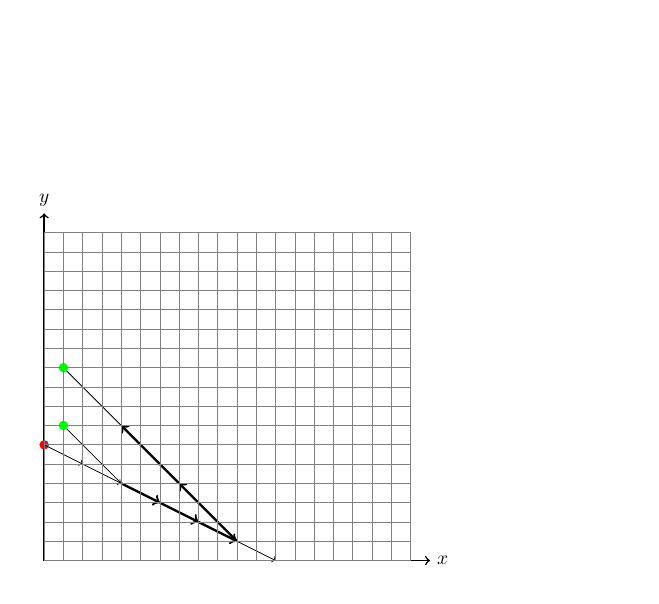
\begin{tikzpicture}[scale=0.35]
\scalebox{0.7}{
\draw[->, thick] (0, 0) -- (20, 0) node[right] {$x$};
\draw[->, thick] (0, 0) -- (0, 18) node[above] {$y$};

\fill[red] (0,6) circle (7pt);

\draw[->] (0,6) -> (2,5);
\draw[->] (2,5) -> (4,4);
\draw[very thick,->] (4,4) -> (6,3);
\draw[very thick,->] (6,3) -> (8,2);
\draw[very thick,->] (8,2) -> (10,1);
\draw[->] (10,1) -> (12,0);

\draw[->] (4,4) -> (1,7);
\fill[green] (1,7) circle (7pt);

\draw[very thick,->] (10,1) -> (7,4);
\draw[very thick,->] (7,4) -> (4,7);
\draw[->] (4,7) -> (1,10);
\fill[green] (1,10) circle (7pt);

\draw[step=1, gray, thin] (0, 0) grid (19, 17);
}
\end{tikzpicture}
\end{minipage}
\begin{minipage}{0.5\textwidth}
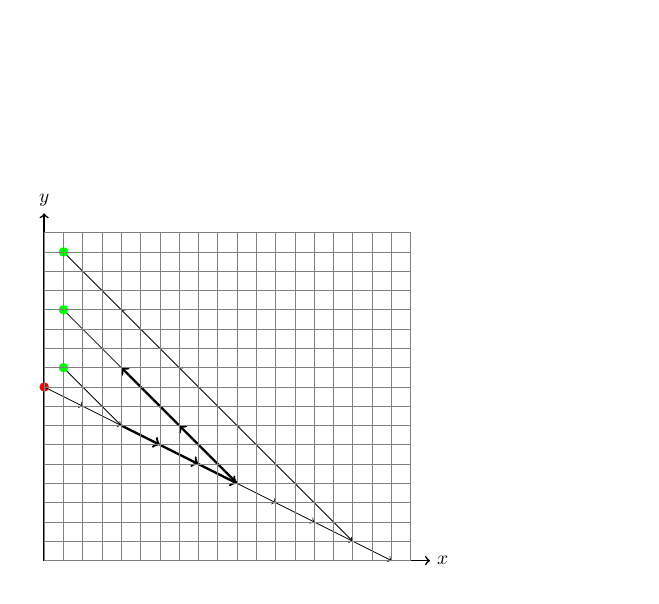
\begin{tikzpicture}[scale=0.35]
\scalebox{0.7}{
\draw[->, thick] (0, 0) -- (20, 0) node[right] {$x$};
\draw[->, thick] (0, 0) -- (0, 18) node[above] {$y$};

\fill[red] (0,9) circle (7pt);

\draw[->] (0,9) -> (2,8);
\draw[->] (2,8) -> (4,7);
\draw[very thick,->] (4,7) -> (6,6);
\draw[very thick,->] (6,6) -> (8,5);
\draw[very thick,->] (8,5) -> (10,4);
\draw[->] (10,4) -> (12,3);
\draw[->] (12,3) -> (14,2);
\draw[->] (14,2) -> (16,1);
\draw[->] (16,1) -> (18,0);

\draw[->] (4,7) -> (1,10);
\fill[green] (1,10) circle (7pt);

\draw[very thick,->] (10,4) -> (7,7);
\draw[very thick,->] (7,7) -> (4,10);
\draw[->] (4,10) -> (1,13);
\fill[green] (1,13) circle (7pt);

\draw[->] (16,1) -> (13,4);
\draw[->] (13,4) -> (10,7);
\draw[->] (10,7) -> (7,10);
\draw[->] (7,10) -> (4,13);
\draw[->] (4,13) -> (1,16);
\fill[green] (1,16) circle (7pt);

\draw[step=1, gray, thin] (0, 0) grid (19, 17);
}
\end{tikzpicture}
\end{minipage}

\caption{Left: $u_2 = 6$, $S_2 = \set{7,10}$. Right: $u_2 = 9$, $S_2 = \set{10,13,16}$.
Thick vectors add up to $p$.}
\label{fig:infix}
\end{figure}

Let $\alpha_1$ and $\alpha_2$ be empty sequences, $\eff(\beta_1) = (2, -1)$ and $\eff(\beta_2) = (-3, 3)$.
Let $u_1 = 0$, $v_1 = 1$. 
The set of solutions $(n_1, n_2)$ of~\eqref{eq:xy} is of the form $w+p^*$, where
$w = (2,1)$ and $p = (3,2)$, and
$\eff_2(p) = 3 \cdot (-1) + 2 \cdot 3 = 3$.
Figure~\ref{fig:infix} shows $R(u_2) = \set{7,10}$ when $u_2 = 6$, and $R(u_2)  = \set{10,13,16}$ when $u_2 = 9$.
In the latter case, elements of $R(u_2)$ correspond to the solutions $w$, $w+p$ and $w+2p$ of~\eqref{eq:xy},
i.e., to $w + kp$ for $k$ in an interval $[0,2]$.
According to Claim~\ref{cl:interval}, this is true in general.
%$S_2 = \setof{u + kp}{k\in I}$, for some interval $I$.
\end{example}

%The following claim states that the number of possible periods $p$ used in the run is an interval.

\begin{claim}\label{cl:interval}
For each $c \in S_1$ there exists an interval $I_{c} = [k_1, k_2]$, where $k_1\in \N$ and $k_2 \in \N_{\infty}$,
such that
$R(c) = \setof{\eff_2(w) + k \cdot \eff_2(p)}{k\in I_{c}}$.
% and path $\rho(b+kp)$ starting from $(b_1, c)$ is a valid if and only if $k \in I_c$. 
\end{claim}

\begin{proof}
It is sufficient to show that whenever $(u_1, c) \trans{w + k_1 \cdot p}$ and
$(u_1, c) \trans{w + k_2 \cdot p}$ for some
$k_1 < k_2 \in \N$,
then
$(u_1, c) \trans{w + k \cdot p}$ for all $k \in [k_1, k_2]$.
Fix $k \in [k_1, k_2]$.
Every point $x$ on the (possibly $\Z$-)path $(u_1, c) \trans{w + k \cdot p}$ is actually on a straight line between some two points,
one on the path $(u_1, c) \trans{w + k_1 \cdot p}$, and the other on the path $(u_1, c) \trans{w + k_2 \cdot p}$.
In consequence $x$, being a weighted average of the two points in $\N^2$, necessarily belongs to $\N^2$. 
Therefore $(u_1, c) \trans{w + k \cdot p}$ is a path.
\end{proof}

We notice that $\eff_2(p)$ can be negative, but this is irrelevant for our arguments.
%
By Claim~\ref{cl:interval}, for each $c \in S_1$ the set $R(c)$ is
is an arithmetic sequence of difference $\essdvass r := \absv{\eff_2(p)}$ and length equal to the cardinality
of the interval $I_{c}$.
%Thus $R(c) = b + (\essdvass r)^{\card{I_c}}$, for some $b\in\N$. 
Let $\spn(c)\in\N_\infty$ be the difference between the supremum of $R(c)$ and the minimal element in $R(c)$.
We say that $\spn(c) = \infty$ if $R(c)$ is infinite.
We split the proof into cases, depending on
whether $\essdvass r$ divides the difference $r$ of the sequence $S_1$, or not.
Additionally we have a case when $\essdvass r = 0$, in other cases we silently assume that $\essdvass r \neq 0$.


\para{Case I: $r$ is divisible by $\essdvass r$}

Therefore, if $\spn(c) \geq r$ then the sequence $R(c)$ actually touches the sequence $R(c+r)$,
i.e., their union is a larger arithmetic sequence of difference $\essdvass r$:

\begin{claim}\label{cl:merged}
If $R(c+r^*) \neq \emptyset$ and $c \geq D:= 3(M+r) \cdot M^2 + M \cdot \norm(w)$,
then $R(c+r^{\leq T}) = b+(\essdvass r)^{\leq T'}$ for some $b \leq c + \eff_2(w) + M \cdot \eff_2(p)$ and $T' \in \N_\infty$.
\end{claim}

\begin{proof}
We first show that $\spn(c) \geq r$.
Suppose $R(c+r^*) \neq \emptyset$ and $c \geq D$.
Due to the first assumption,  for some $n\in\N$ there is a path $(u_1, c+nr) \trans{(n_1, n_2)}$
of the form
\begin{align} \label{eq:Mp}
(u_1, c+nr) \trans{\alpha_1} (\essdvass{x}_1, \essdvass{y}_1) \trans{\beta_1^{n_1}} (\essdvass{x}_2, \essdvass{y}_2) \trans{\alpha_2} (\essdvass{x}_3, \essdvass{y}_3) \trans{\beta_2^{n_2}} (v_1, v_2).
\end{align}
In particular,  $u_1 \geq \drop_1(\alpha_1)$
and therefore $\essdvass x_1\geq 0$.
It is enough to take $(n_1, n_2) := w + Mp$ in \eqref{eq:Mp}.
Then $n_1 \geq M$, so $\essdvass x_2 \geq \essdvass x_1 + M \geq M \geq \drop_1(\alpha_2)$.
Therefore $\essdvass x_3\geq 0$.
Now we show that $c$ is large enough such that $(u_1, c) \trans{w+Mp}$ is nonnegative on the second coordinate as well.
As $\norm(p) \leq 2M$ then $n_1 + n_2 \leq M \cdot \norm(p) + \norm(w) \leq 2M^2 + \norm(w)$. Therefore
$\beta_1^{n_1}$ and $\beta_2^{n_2}$ can in total decrease the second coordinate by at most $M \cdot (2M^2 + \norm(w))$.
As $\alpha_1 + \alpha_2$ can in total decrease the second coordinate by at most $M$ and
$D \geq M + M \cdot (2M^2 + \norm(w))$ we conclude that indeed the path $(u_1, c) \trans{w+Mp}$ is valid.
For the same reasons, for every $m\in [M, M+r]$ there is a path $(u_1, c) \trans{w+mp}$, which guarantees $\spn(c) \geq r$. 

Now we use that fact that $\spn(c) \geq r$.
By monotonicity of \vass, if $R(c) = b+(\essdvass r)^{\leq {T'}}$
then $R(c+r)$ necessarily includes $R(c) + r= b+r+(\essdvass r)^{\leq {T'}}$.
Since $\spn(c) \geq r$, we have $b+r \in R(c)$, but also $b+r \in R(c+r)$,
and therefore the union $R(c) \cup R(c + r)$ forms one arithmetic sequence 
$b+(\essdvass r)^{\leq T'}$, for some $b\in\N$ and $T'$.
The similar reasoning applies to any finite union, namely to $R(c+r^{\leq m})$ for $m\in\N$.
In consequence, for every $T\in \N_\infty$ we have $R(c+r^{\leq T}) = b + (\essdvass r)^{\leq T'}$,
for some $b\in\N$ and $T'\in \N_\infty$,
and since $c+ \eff_2(w) + M \cdot \eff_2(p) \in R(c)$ we get the inequality $b \leq c + \eff_2(w) + M \cdot \eff_2(p)$, as required.
\end{proof}

We are ready for concluding Case I.
%Let $D = 3(M+r) \cdot M^2 + M \cdot \norm(w)$, as in the Claim~\ref{cl:bigspan}.
As $\norm(w) \leq \poly(B, M)$ we have $D \leq \poly(B, M, r)$.
We  partition $S_1 = a + r^{\leq T}$ into two subsets: $S'_1 = S_1 \cap [0,D)$
and $S''_1 = S_1 \cap [D,\infty)$, both being arithmetic sequences of difference $r$,
and consider $S'_1$ and $S''_1$ separately.
 
Concerning $S'_2:= R(S'_1)$,
as $\max(S'_1) \leq D$, all
elements of $S'_2$ are upper-bounded by a polynomial in $M$ and $r$, namely
$\max(S'_2) \leq M^2 \cdot (2M + D)$. 
Thus $S'_2$ can be seen as a finite sum of singletons, each of which
being an $(a', r', T')$-arithmetic sequence with $a' \leq M^2 \cdot (2M + D) \leq \poly(B,M,r)$,
$r' = 1$ and $T' = 0$. 
Clearly $r' = 1 \leq \poly(M)$, and hence $S'_2$ is of the required form.

Now we consider $S''_2:= R(S''_1)$.
If $S''_2 = \emptyset$ we are done.
Otherwise, let $c:= \min(S''_1)$.
Thus $S''_1 = c+r^{\leq T}$ for some $T \in \N_\infty$, 
and $D\leq c \leq \max(a, D+r)$.
%By Claim~\ref{cl:bigspan}, $\spn(c) \geq r$, and therefore using Claim~\ref{cl:neighbours} 
By Claim~\ref{cl:merged} we deduce that
$S''_2 = b + (\essdvass r)^{\leq T'}$ for some 
$b \leq c + \eff_2(w) + M \cdot \eff_2(p)$ and $T' \in \N_\infty'$. 
As $\eff_2(w) \leq \poly(B,M)$, $\eff_2(p) \leq \poly(M)$ and $c \leq a + \poly(B,M, r)$ we get $b \leq a + \poly(B, M, r)$.
We also have $\essdvass r \leq \poly(M)$, and hence
$S''_2$ is of the required form.


\para{Case II: $r$ is not divisible by $\essdvass r$}
%Assume now that $r$ does not divide $\eff_2(p)$. 

In that case we split $S_1 = a + r^{\leq T}$ into several
arithmetic sequences of difference $r \cdot \essdvass r$, namely into sequences of a form 
$(a + m \cdot r) + (r \cdot \essdvass r)^{\leq T'}$, where $m < \essdvass r$, 
and apply the above reasoning to each of this sequences separately. 
As $\essdvass r \leq \poly(M)$
we get also a finite set of arithmetic sequences with the base bounded by $a + \poly(B, M,r)$ and difference bounded by $\poly(M)$,
as required.

\para{Case III: $\essdvass r = 0$}
\Wlog we assume $R(S_1) \neq \emptyset$. For every $c \in S_1$ we have that either $R(c) = c + \eff_2(w)$ or $R(c) = \emptyset$. By monotonicity of VASS we have that if $R(c) \neq \emptyset$ then $R(c+r) \neq \emptyset$. Let $D := 3(M+r) \cdot M^2 + M \cdot \norm(w)$. Similarly as in the proof of Claim~\ref{cl:merged} we observe that if $c \geq D$ then for some $k \in N$ there is a run $(u_1, c) \trans{w+kp}$. Hence we have $R(S_1) = c + \eff_2(w) + r^{\leq T'}$ for some $T' \in \N_\infty$ and some $c \in S_1$ such that $c \leq \max(a, D+r)$. Therefore $R(S_1) = b + r^{\leq T'}$ for some $b \leq a + \poly(B,M,r)$ as required.

\end{proof}



%
%Observe, that if $(b_1, s) \trans \rho (b_2, t)$ for $s \in S_1$ and $t \in S_2$ then $x,y$ satisfy the following equation:
%$$\eff_1(\alpha_1\alpha_2) + x\eff_1(\beta_1) + y\eff_1(\beta_2) = b_2-b_1$$
%Hence we have that the set $S$ of such  pairs $(x,y)$ associated is included in set of solutions of the above equation, which can be represented by Lemma~\ref{lem:taming} as $L(B,P)$ for some sets $B, P \subseteq \N^2$ such that $\norm(B) \leq c(M+B)$ and $\norm(P) \leq cM$ for some constant $c \in \N_+$. We show, that $P$ has only one element $p$. This is because the set of solutions of the following equations over $\Q$ is one dimensional vector space and there is nonnegative solution, because of different signs of $\eff_1(\beta_1)$ and $\eff_1(\beta_2)$:
%$$x\eff_1(\beta_1) + y\eff_1(\beta_2) = 0$$
%Hence each path can be represented as $b+kp$ for some $k \in \N$ and $b \in B$ (recall that with each path we associated pair $(x,y)$). Because $B$ is finite and we are interested in a finite union representation it is enough to show that there exists polynomial $R(M)$ such that the set $S_2' =   \{y_2 \mid \exists_{y_1 \in S_1} (b_1, y_1) \trans{b+kp} (b_2, y_2), k \in \N \}$ is a finite union of $(a', r', T')$-arithmetic sets with $a' \leq a + (B+r) \cdot R(M)$ and
%$r' \leq R(M)$.
%
%We have $p=(p_1, p_2)$ and we write $\eff(p)$ for $\eff(\beta_1^{p_1}\beta_2^{p_2})$. Moreover $b = (b_1, b_2)$ and we write $\eff(b+kp)$ for $\eff(\alpha_1\beta_1^{b_1}\alpha_2\beta_2^{b_2}) + k \eff(p)$. First we solve a case when $|\eff_2(p)|$ divides $r$, to which we will reduce the other case. Let $m = \frac{r}{|\eff_2(p)|}$. Moreover, \mywlog we can assume that $S_2' \neq \emptyset$.
%The intuition is that the set $S_2'$ will be a condensing of $S_1$ due to repetitions of $p$ with base point $a'$ moved a bit. In order to conclude the prove we need a few claims. 
%\begin{claim}
%For each $s \in S_1$ there exists interval $I = [k_1, k_2]$ such that $k_1, k_2 \in \N_{\infty}$ and path $b+kp$ starting from $s$ is a valid path if and only if $k \in I$. 
%\end{claim}
%\begin{proof}
%It is enough to show, that if for $k_1 < k_2 \in \N$ we know, that $b+k_1p$ and $b+k_2p$ are valid paths starting from $s$ then for all $k_3 \in [k_1, k_2]$ we have that path $b+k_3p$ is a valid path starting from $s$. Let us fix $k_3 \in [k_1, k_2]$ and let $b=(b_1, b_2), p=(p_1, p_2) \in \N^2$. Recall, that $\eff(\beta_1) \in \N_+ \times \N_-$ and $\eff(\beta_2) \in \N_- \times \N_+$. Hence it is enough to show the following inequalities:
%$$\eff_1(\alpha_1\beta_1^{b_1+k_3p_1}\alpha_2\beta_2^{b_2+k_3p_2}) = \eff_1(\alpha_1\beta_1^{b_1+k_1p_1}\alpha_2\beta_2^{b_2+k_1p_2})$$
%$$\eff_2(\alpha_1\beta_1^{b_1+k_3p_1}) \geq \eff_2(\alpha_1\beta_1^{b_1+k_2p_1})$$
%For the first equality observe, that:
%\begin{align*}
%\eff_1(\alpha_1\beta_1^{b_1+k_3p_1}\alpha_2\beta_2^{b_2+k_3p_2}) & = \eff_1(\alpha_1\beta_1^{b_1+k_1p_1}\alpha_2\beta_2^{b_2+k_1p_2}) 
%+ (k_3-k_1)(p_1\eff_1(\beta_1) + p_2\eff_1(\beta_2)) \\
%& = \eff_1(\alpha_1\beta_1^{b_1+k_1p_1}\alpha_2\beta_2^{b_2+k_1p_2})
%\end{align*}
%The second inequality follows from the fact that:
%$$b_1+k_3p_1 \leq b_1+k_2p_1$$
%\end{proof}
%Let us by $I_x = [k_1^s, k_2^s]$ denote the interval for $x \in S_1$ and by $|I_x| = k_2^s - k_1^s$. Now we split elements of $S_1$ into three groups depending on the properties of the points in $S_1$.
%\begin{claim}\label{clm:split}
%For each $x \in S_1$ at least one of the following holds:
%\begin{itemize}
%\item $x \leq a + 3cM^2(B+r)$
%\item $x$ is the maximal element of $S_1$ and $[0,m] \subseteq I_x$
%\item $[0, m] \subseteq I_x$ and if $b+kp$ is executable from $(b_1,x)$ for $k > m$ than $b+(k-m)p$ is executable from $(b_1,x+m\eff_2(p))$ and $x+m\eff_2(p) \in S_1$. 
%\end{itemize}
%\end{claim}
%\begin{proof}
%Let us take $x \in S_1$ such that  $x > a + 3cM^2(B+r)$. Firstly, we show that $[0, m] \subseteq I_x$. Recall, that $\Lambda$ is one-turn and observe, that for all $k \in \N$ we have:
%$$\eff_1(\alpha_1\beta_1^{b_1}\alpha_2\beta_2^{b_2}) = \eff_1(\alpha_1\beta_1^{b_1}\alpha_2\beta_2^{b_2}) + k(p_1\eff_1(\beta_1) + p_2\eff_1(\beta_2))$$
%Hence, because $S_2$ is not empty we have that all paths $b+kp$ starting from $(b_1, x)$ are valid on the first counter. Hence we only need to deal with the second counter. Now observe, that for each $k \in [0,m]$ we have that maximal decrease of the second counter along path $b+kp$ is at most :
%\begin{align*}
%M + (b_1+kp_1)\eff_2(\beta_1) & \leq M + (c(M+B)+mcM)M \\
%& \leq 3cM^2(B+m) \leq 3CM^2(B+r) < x
%\end{align*}
%Hence $[0, m] \subseteq I_x$.
%If $x$ is the maximal element we are done. Otherwise,
%we show, that if $b+kp$ is executable from $(b_1,x)$ for $k > m$ than $b+(k-m)p$ is executable from $(b_1,x+m\eff_2(p))$ and $x+m\eff_2(p) \in S_1$. Observe, that $x+m\eff_2(p) = x+r$ if $\eff_2(p) > 0$ and $x+m\eff_2(p) = x-r$ otherwise. Because $S_1 =  a + r^{\leq K}$ and $x$ is not the maximal element of $S_1$ then in the first case $x+m\eff_2(p) \in S_1$. In the second case we have $x -  r \geq a+r-r \geq a$ and hence $x-r \in S_1$.
%
%Now it is left, that $b+(k-m)p$ is executable from $(b_1,x+m\eff_2(p))$. Similarly as before we only need to take care about the second counter. For this it is enough to observe, that:
%\begin{align*}
%x + m\eff_2(p) + \eff_2(\alpha_1\beta_1^{b_1+(k-m)p_1}) 
%& = x + \eff_2(\alpha_1\beta_1^{b_1+kp_1}) + mp_2\eff_2(\beta_2) \\
%& \geq x + \eff_2(\alpha_1\beta_1^{b_1+kp_1})
%\end{align*}
%This is due to $\eff_2(p) = p_1\eff_2(\beta_1) + p_2\eff_2(\beta_2)$ and $\eff_2(\beta_2) \geq 0$.
%Moreover:
%$$x+m\eff_2(p) \geq a+3cM^2(B+r)-r \geq a + M \geq |\eff_2(\alpha_1)|$$
%\end{proof}
%Now we can split $S_1$ into three parts $A_1, A_2, A_3$ such that elements from $A_1$ are the one with $s \leq a + 3cM^2(B+r)$, $A_3$ is the singleton or empty set containing the maximal element and $A_2$ is the rest of $S_1$. Observe, that $A_2 = a_2+r^{\leq K}$ for $a_2 \leq 3cM^2(B+r) + r, a_2 = a + kr$ for some $k \in \N$ and $K = T - k - 1$. Moreover observe, that if path start from $s \in A_2$ and is of the form $b+kp$ for $k > m$ than the same point is reachable from point $(b_1,s+m\eff_2(p))$ by path $b+(k-m)p$ due to Claim \ref{clm:split}. Hence, because we can iterate the argument at some point the starting point will be in $A_1 \cup A_3$ or $k \leq m$. Hence for points from $A_2$ we only need to consider paths $b+kp$ for $k \leq m$. Let us define $B_1, B_2$ and $B_3$.  
%$$B_1 = \bigcup_{x \in A_1, k \in I_x} \set{x + \eff_2(b+kp)}$$
%$$B_2 = \bigcup_{x \in A_2, k \in [0,m]} \set{x + \eff_2(b+kp)} 
%= a_2 + r^{\leq T} + \eff_2(b) + \eff_2(p)^{\leq m}$$
%$$B_3 = \bigcup_{x \in A_3, k \in I_s} \set{x + \eff_2(b+kp)}$$ 
%Which if $A_3 \neq \emptyset$ can be represented as
%$$B_3= a + (T+1)r  + \eff_2(b) + \eff_2(p)^{\leq |I_{x_{max}}|}$$
%where $x_{max}$ is the element of $A_3$. From now on we fix this maximal element and put $|I_{x_max}| = 0$ if it does not exist. 
%Let us observe:
%$$S_2 = B_1 \cup B_2 \cup B_3$$
%We deal separately with $B_1$ and $B_2 \cup B_3$. Because $a_2 + \eff_2(b) \leq 3cM^2(B+r) + r $ clearly, in order to show, that $B_2 \cup B_3$ is  of the form we want it is enough to show the following claim (recall that $\eff_2(p)$ can not be zero due to divisibility condition):
%\begin{claim}
%$(B_2 \cup B_3) \cap [a_2 + \eff_2(b), \infty] = a_2 + \eff_2(b) + |\eff_2(p)|^{\leq T'}$ where $T' = m(T+1) + |I_{x_{max}}|$ if $\eff_2(p) > 0$ and $T' = m(T+1)$ if $\eff_2(p) < 0$ .  
%\end{claim}
%\begin{proof}
%Firstly we show $(B_2 \cup B_3) \cap [a_2 + \eff_2(b), \infty] \subseteq a_2 + \eff_2(b) + |\eff_2(p)|^{\leq T'}$. Let us take any $x \in (B_2 \cup B_3) \cap [a_2 + \eff_2(b), \infty]$. The first case is that $x \in B_2$ and hence 
%$$x = a_2 + \eff_2(b) + k_1r + k_2\eff_2(p)$$
%for $k_1 \leq T$ and $k_2 \leq m$. We have 
%$$x = a_2 + \eff_2(b) + k_1m|\eff_2(p)| + k_2\eff_2(p)$$
%and hence if $\eff_2(p) > 0$ we have 
%$$x = a_2 + \eff_2(b) + (k_1m + k_2)|\eff_2(p)| \in a_2 + \eff_2(b) + |\eff_2(p)|^{\leq T'}$$
%and if $\eff_2(p) < 0$ we have 
%$$x =  a_2 + \eff_2(b) + |\eff_2(p)|^{k_1m-k_2}$$
%Because $x \geq a_2 + \eff_2(b)$ we have $k_1m-k_2 \geq 0$ and hence $x \in a_2 + \eff_2(b) + |\eff_2(p)|^{\leq T'}$ .
%
%Now we show $a_2 + \eff_2(b) + |\eff_2(p)|^{\leq T'} \subseteq (B_2 \cup B_3) \cap [a_2 + \eff_2(b), \infty]$. Let us take $x = a_2 + \eff_2(b) + k|\eff_2(p)|$ for some $k \leq T'$. Firstly let us consider case when $\eff_2(p) > 0$. 
%\begin{align*}
%x & = a_2 + \eff_2(b) + \floor{\frac{k}{m}}m|\eff_2(p)|+ (k\mod m)|\eff_2(p)| \\
%& = a_2 + \eff_2(b) + \floor{\frac{k}{m}}r + (k \mod m)\eff_2(p)
%\end{align*}
%Observe, that if $k \leq m(T+1)$ we have
%$$\floor{\frac{k}{m}} \leq \floor{\frac{m(T+1)}{m}} = T+1$$
%Hence $x \in a_2 + \eff_2(b) + r^{\leq T} + |\eff_2(p)|^{\leq m} = B_2$
%If $k > m(T+1)$ then observe, that $k - m(T+1) \leq |I_{x_{max}}|$ and see, that
%$$x = a_2 + \eff_2(b) + r(T+1) + \eff_2(p)^{k-m(T+1)} \in B_3 $$
%
%Now we consider case when $\eff_2(p) < 0$. Then:
%$$x=a_2 + \eff_2(b) + \ceil{\frac{k}{m}}m|\eff_2(p)|-(m - (k \mod m))|\eff_2(p)|$$
%Then if $k \leq mT$ we have:
%$$x \in a_2 + \eff_2(b) + r^{\leq T}+\eff_2(p)^{\leq m} = B_2 $$
%And if $k > mT$ we have:
%$$x \in a_2 + \eff_2(b) + (T+1)r + \eff_2(p)^{\leq m} \subseteq B_3$$
%
%\end{proof}
%For the set $B_1$ it is enough to prove the following Claim:
%\begin{claim}
%$B_1$ can be represented as a finite union of $(a', r',T')$-arithmetic sets with $a' \leq a + 10cM^4(B+r)$ and $r' \leq cM$.
%\end{claim}
%\begin{proof}
%The first case is that the second counter is at most $3cM^2(B+r)$ at the beginning. The first counter is at most $B$ at the beginning. Then after $\alpha_1$ they are at most $3cM^2(B+r) + M \leq 4cM^2(B+r)$. Then after all execution of the $\beta_1$ the sum of the counters is at most $8cM^3(B+r)$ then after $\alpha_2$ the sum of counters is at most $8cM^3(B+r) + 2M$ and finally after the last execution of $\beta_2$ the sum of counters and hence also the second counter is at most $8cM^4(B+r) + 2M^2 \leq 10cM^4(B+r)$ as needed. Hence there is a finite number of such elements and they can be represented as a singleton arithmetic sets.
%The second case is that the second counter is at least $3cM^2(B+r)$ at the beginning. Let the beginning point be $x$. We show, that elements of $B_1$ obtained by the paths starting in $x$ can be represented as an arithmetic-set. Therefore assume this set is not empty (otherwise it is trivial). Recall, that $\Lambda$ is one-turn and observe, that for all $k \in \N$ we have:
%$$\eff_1(\alpha_1\beta_1^{b_1}\alpha_2\beta_2^{b_2}) = \eff_1(\alpha_1\beta_1^{b_1}\alpha_2\beta_2^{b_2}) + k(p_1\eff_1(\beta_1) + p_2\eff_1(\beta_2))$$
%All paths $b+kp$ starting from $x$ are valid on the first counter. Hence we only need to deal with the second counter. Now observe, that  we have that maximal decrease of the second counter along path $b$ is at most :
%$$M + b_1\eff_2(\beta_1) \leq M + c(M+B)M \leq 3cM^2B$$ Hence path $b$ is also valid on the second counter. Hence $x_2 + \eff_2(b) \in B_1$ and $x_2 + \eff_2(b) \leq a + 3cM^2(B+r) + \eff_2(\alpha_1\alpha_2) + b_1\eff_2(\beta_1) + b_2\eff_2(\beta_2) \leq a + 3cM^2(B+r) + M +  2c(M+B)M \leq a + 10cM^2(B+r)$. Now if $\eff_2(p) > 0$ then the set can be represented as $(x_2 + \eff_2(b), \eff_2(p), T')$-arithmetic set, which satisfies the conditions. Otherwise all elements are at most $a + 10cM^2(B+r)$ and can be represented as singleton arithmetic sets, which satisfies the conditions.
%\end{proof}
%By previous claims we know, that $S_2$ is a finite union of $(a',r', T')$-arithmetic sets for $a' \leq a + 10cM^4(B+r)$ and $r' \leq cM$.
%
%
%Now we come back to the case when $r$ is not divisible by $|\eff_2(p)|$. The first subcase is that $\eff_2(p) = 0$. Then all paths $b+kp$ have the same effect so we only need to consider path $b$. The lowest $x \in S_1$ from which the path $b$ is executable is at most $M + b_1\eff_2(\beta_1) + a + r \leq M + c(M+B)M + a+r \leq a + 3M^2(B+r)$. Hence set $S_2$ can be represented as $(a', r, T')$-arithmetic set for $a' \leq a+ 3M^2(B+r) + \eff_2(b) \leq a+ 3M^2(B+r) + M+2c(M+B)M \leq a + 10M^2(B+r)$. The second subcase is that $\eff_2(p) \neq 0$. Then we can split $S_1$ into several $(a'', \eff_2(p)r, T'')$-arithmetic sets with $a'' \leq a + \eff_2(p)r \leq a + (2cM^2+M)r$ then we can apply the first case and get representation of $S_2$ as a finite union of $(a',r', T')$-arithmetic sets with $r' \leq cM$ and $a' \leq a + (2cM^2+M)r + 10cM^4(B+r) \leq a+ 13M^4(B+r)$. Thus by setting $R(M) = 13cM^4$ we conclude the proof. 
%\end{proof}

\section{Discussion of Assumptions}\label{sec:discussion}
In this paper, we have made several assumptions for the sake of clarity and simplicity. In this section, we discuss the rationale behind these assumptions, the extent to which these assumptions hold in practice, and the consequences for our protocol when these assumptions hold.

\subsection{Assumptions on the Demand}

There are two simplifying assumptions we make about the demand. First, we assume the demand at any time is relatively small compared to the channel capacities. Second, we take the demand to be constant over time. We elaborate upon both these points below.

\paragraph{Small demands} The assumption that demands are small relative to channel capacities is made precise in \eqref{eq:large_capacity_assumption}. This assumption simplifies two major aspects of our protocol. First, it largely removes congestion from consideration. In \eqref{eq:primal_problem}, there is no constraint ensuring that total flow in both directions stays below capacity--this is always met. Consequently, there is no Lagrange multiplier for congestion and no congestion pricing; only imbalance penalties apply. In contrast, protocols in \cite{sivaraman2020high, varma2021throughput, wang2024fence} include congestion fees due to explicit congestion constraints. Second, the bound \eqref{eq:large_capacity_assumption} ensures that as long as channels remain balanced, the network can always meet demand, no matter how the demand is routed. Since channels can rebalance when necessary, they never drop transactions. This allows prices and flows to adjust as per the equations in \eqref{eq:algorithm}, which makes it easier to prove the protocol's convergence guarantees. This also preserves the key property that a channel's price remains proportional to net money flow through it.

In practice, payment channel networks are used most often for micro-payments, for which on-chain transactions are prohibitively expensive; large transactions typically take place directly on the blockchain. For example, according to \cite{river2023lightning}, the average channel capacity is roughly $0.1$ BTC ($5,000$ BTC distributed over $50,000$ channels), while the average transaction amount is less than $0.0004$ BTC ($44.7k$ satoshis). Thus, the small demand assumption is not too unrealistic. Additionally, the occasional large transaction can be treated as a sequence of smaller transactions by breaking it into packets and executing each packet serially (as done by \cite{sivaraman2020high}).
Lastly, a good path discovery process that favors large capacity channels over small capacity ones can help ensure that the bound in \eqref{eq:large_capacity_assumption} holds.

\paragraph{Constant demands} 
In this work, we assume that any transacting pair of nodes have a steady transaction demand between them (see Section \ref{sec:transaction_requests}). Making this assumption is necessary to obtain the kind of guarantees that we have presented in this paper. Unless the demand is steady, it is unreasonable to expect that the flows converge to a steady value. Weaker assumptions on the demand lead to weaker guarantees. For example, with the more general setting of stochastic, but i.i.d. demand between any two nodes, \cite{varma2021throughput} shows that the channel queue lengths are bounded in expectation. If the demand can be arbitrary, then it is very hard to get any meaningful performance guarantees; \cite{wang2024fence} shows that even for a single bidirectional channel, the competitive ratio is infinite. Indeed, because a PCN is a decentralized system and decisions must be made based on local information alone, it is difficult for the network to find the optimal detailed balance flow at every time step with a time-varying demand.  With a steady demand, the network can discover the optimal flows in a reasonably short time, as our work shows.

We view the constant demand assumption as an approximation for a more general demand process that could be piece-wise constant, stochastic, or both (see simulations in Figure \ref{fig:five_nodes_variable_demand}).
We believe it should be possible to merge ideas from our work and \cite{varma2021throughput} to provide guarantees in a setting with random demands with arbitrary means. We leave this for future work. In addition, our work suggests that a reasonable method of handling stochastic demands is to queue the transaction requests \textit{at the source node} itself. This queuing action should be viewed in conjunction with flow-control. Indeed, a temporarily high unidirectional demand would raise prices for the sender, incentivizing the sender to stop sending the transactions. If the sender queues the transactions, they can send them later when prices drop. This form of queuing does not require any overhaul of the basic PCN infrastructure and is therefore simpler to implement than per-channel queues as suggested by \cite{sivaraman2020high} and \cite{varma2021throughput}.

\subsection{The Incentive of Channels}
The actions of the channels as prescribed by the DEBT control protocol can be summarized as follows. Channels adjust their prices in proportion to the net flow through them. They rebalance themselves whenever necessary and execute any transaction request that has been made of them. We discuss both these aspects below.

\paragraph{On Prices}
In this work, the exclusive role of channel prices is to ensure that the flows through each channel remains balanced. In practice, it would be important to include other components in a channel's price/fee as well: a congestion price  and an incentive price. The congestion price, as suggested by \cite{varma2021throughput}, would depend on the total flow of transactions through the channel, and would incentivize nodes to balance the load over different paths. The incentive price, which is commonly used in practice \cite{river2023lightning}, is necessary to provide channels with an incentive to serve as an intermediary for different channels. In practice, we expect both these components to be smaller than the imbalance price. Consequently, we expect the behavior of our protocol to be similar to our theoretical results even with these additional prices.

A key aspect of our protocol is that channel fees are allowed to be negative. Although the original Lightning network whitepaper \cite{poon2016bitcoin} suggests that negative channel prices may be a good solution to promote rebalancing, the idea of negative prices in not very popular in the literature. To our knowledge, the only prior work with this feature is \cite{varma2021throughput}. Indeed, in papers such as \cite{van2021merchant} and \cite{wang2024fence}, the price function is explicitly modified such that the channel price is never negative. The results of our paper show the benefits of negative prices. For one, in steady state, equal flows in both directions ensure that a channel doesn't loose any money (the other price components mentioned above ensure that the channel will only gain money). More importantly, negative prices are important to ensure that the protocol selectively stifles acyclic flows while allowing circulations to flow. Indeed, in the example of Section \ref{sec:flow_control_example}, the flows between nodes $A$ and $C$ are left on only because the large positive price over one channel is canceled by the corresponding negative price over the other channel, leading to a net zero price.

Lastly, observe that in the DEBT control protocol, the price charged by a channel does not depend on its capacity. This is a natural consequence of the price being the Lagrange multiplier for the net-zero flow constraint, which also does not depend on the channel capacity. In contrast, in many other works, the imbalance price is normalized by the channel capacity \cite{ren2018optimal, lin2020funds, wang2024fence}; this is shown to work well in practice. The rationale for such a price structure is explained well in \cite{wang2024fence}, where this fee is derived with the aim of always maintaining some balance (liquidity) at each end of every channel. This is a reasonable aim if a channel is to never rebalance itself; the experiments of the aforementioned papers are conducted in such a regime. In this work, however, we allow the channels to rebalance themselves a few times in order to settle on a detailed balance flow. This is because our focus is on the long-term steady state performance of the protocol. This difference in perspective also shows up in how the price depends on the channel imbalance. \cite{lin2020funds} and \cite{wang2024fence} advocate for strictly convex prices whereas this work and \cite{varma2021throughput} propose linear prices.

\paragraph{On Rebalancing} 
Recall that the DEBT control protocol ensures that the flows in the network converge to a detailed balance flow, which can be sustained perpetually without any rebalancing. However, during the transient phase (before convergence), channels may have to perform on-chain rebalancing a few times. Since rebalancing is an expensive operation, it is worthwhile discussing methods by which channels can reduce the extent of rebalancing. One option for the channels to reduce the extent of rebalancing is to increase their capacity; however, this comes at the cost of locking in more capital. Each channel can decide for itself the optimum amount of capital to lock in. Another option, which we discuss in Section \ref{sec:five_node}, is for channels to increase the rate $\gamma$ at which they adjust prices. 

Ultimately, whether or not it is beneficial for a channel to rebalance depends on the time-horizon under consideration. Our protocol is based on the assumption that the demand remains steady for a long period of time. If this is indeed the case, it would be worthwhile for a channel to rebalance itself as it can make up this cost through the incentive fees gained from the flow of transactions through it in steady state. If a channel chooses not to rebalance itself, however, there is a risk of being trapped in a deadlock, which is suboptimal for not only the nodes but also the channel.

\section{Conclusion}
This work presents DEBT control: a protocol for payment channel networks that uses source routing and flow control based on channel prices. The protocol is derived by posing a network utility maximization problem and analyzing its dual minimization. It is shown that under steady demands, the protocol guides the network to an optimal, sustainable point. Simulations show its robustness to demand variations. The work demonstrates that simple protocols with strong theoretical guarantees are possible for PCNs and we hope it inspires further theoretical research in this direction.
\section{Related Works}
\label{sec:related_works}


\noindent\textbf{Diffusion-based Video Generation. }
The advancement of diffusion models \cite{rombach2022high, ramesh2022hierarchical, zheng2022entropy} has led to significant progress in video generation. Due to the scarcity of high-quality video-text datasets \cite{Blattmann2023, Blattmann2023a}, researchers have adapted existing text-to-image (T2I) models to facilitate text-to-video (T2V) generation. Notable examples include AnimateDiff \cite{Guo2023}, Align your Latents \cite{Blattmann2023a}, PYoCo \cite{ge2023preserve}, and Emu Video \cite{girdhar2023emu}. Further advancements, such as LVDM \cite{he2022latent}, VideoCrafter \cite{chen2023videocrafter1, chen2024videocrafter2}, ModelScope \cite{wang2023modelscope}, LAVIE \cite{wang2023lavie}, and VideoFactory \cite{wang2024videofactory}, have refined these approaches by fine-tuning both spatial and temporal blocks, leveraging T2I models for initialization to improve video quality.
Recently, Sora \cite{brooks2024video} and CogVideoX \cite{yang2024cogvideox} enhance video generation by introducing Transformer-based diffusion backbones \cite{Peebles2023, Ma2024, Yu2024} and utilizing 3D-VAE, unlocking the potential for realistic world simulators. Additionally, SVD \cite{Blattmann2023}, SEINE \cite{chen2023seine}, PixelDance \cite{zeng2024make} and PIA \cite{zhang2024pia} have made significant strides in image-to-video generation, achieving notable improvements in quality and flexibility.
Further, I2VGen-XL \cite{zhang2023i2vgen}, DynamicCrafter \cite{Xing2023}, and Moonshot \cite{zhang2024moonshot} incorporate additional cross-attention layers to strengthen conditional signals during generation.



\noindent\textbf{Controllable Generation.}
Controllable generation has become a central focus in both image \citep{Zhang2023,jiang2024survey, Mou2024, Zheng2023, peng2024controlnext, ye2023ip, wu2024spherediffusion, song2024moma, wu2024ifadapter} and video \citep{gong2024atomovideo, zhang2024moonshot, guo2025sparsectrl, jiang2024videobooth} generation, enabling users to direct the output through various types of control. A wide range of controllable inputs has been explored, including text descriptions, pose \citep{ma2024follow,wang2023disco,hu2024animate,xu2024magicanimate}, audio \citep{tang2023anytoany,tian2024emo,he2024co}, identity representations \citep{chefer2024still,wang2024customvideo,wu2024customcrafter}, trajectory \citep{yin2023dragnuwa,chen2024motion,li2024generative,wu2024motionbooth, namekata2024sg}.


\noindent\textbf{Text-based Camera Control.}
Text-based camera control methods use natural language descriptions to guide camera motion in video generation. AnimateDiff \cite{Guo2023} and SVD \cite{Blattmann2023} fine-tune LoRAs \cite{hu2021lora} for specific camera movements based on text input. 
Image conductor\cite{li2024image} proposed to separate different camera and object motions through camera LoRA weight and object LoRA weight to achieve more precise motion control.
In contrast, MotionMaster \cite{hu2024motionmaster} and Peekaboo \cite{jain2024peekaboo} offer training-free approaches for generating coarse-grained camera motions, though with limited precision. VideoComposer \cite{wang2024videocomposer} adjusts pixel-level motion vectors to provide finer control, but challenges remain in achieving precise camera control.

\noindent\textbf{Trajectory-based Camera Control.}
MotionCtrl \cite{Wang2024Motionctrl}, CameraCtrl \cite{He2024Cameractrl}, and Direct-a-Video \cite{yang2024direct} use camera pose as input to enhance control, while CVD \cite{kuang2024collaborative} extends CameraCtrl for multi-view generation, though still limited by motion complexity. To improve geometric consistency, Pose-guided diffusion \cite{tseng2023consistent}, CamCo \cite{Xu2024}, and CamI2V \cite{zheng2024cami2v} apply epipolar constraints for consistent viewpoints. VD3D \cite{bahmani2024vd3d} introduces a ControlNet\cite{Zhang2023}-like conditioning mechanism with spatiotemporal camera embeddings, enabling more precise control.
CamTrol \cite{hou2024training} offers a training-free approach that renders static point clouds into multi-view frames for video generation. Cavia \cite{xu2024cavia} introduces view-integrated attention mechanisms to improve viewpoint and temporal consistency, while I2VControl-Camera \cite{feng2024i2vcontrol} refines camera movement by employing point trajectories in the camera coordinate system. Despite these advancements, challenges in maintaining camera control and scene-scale consistency remain, which our method seeks to address. It is noted that 4Dim~\cite{watson2024controlling} introduces absolute scale but in  4D novel view synthesis (NVS) of scenes.




\section{Dataset and Training Details}
\label{app:dataset_n_train}

\subsection{Dataset Generation for Offline Training}
\begin{figure}[t]
    \centering
    \includegraphics[width=\linewidth]{images/entity_label.pdf}
    \vspace{-1.5pc}
    \caption{Illustration of our entity-level dataset construction. We form entity-level hallucination labels according to the atomic facts extracted by \textsc{FActScore}.}
    \label{fig:data_generation}
    \vspace{-1pc}
\end{figure}

The Multiturn-aware Reward (MR) function enables the generation of high-quality synthetic conversation datasets for training. Given a user query, multiple LLM responses are sampled and ranked based on their MR scores, with higher-ranked responses designated as \textit{Chosen} and lower-ranked as \textit{Rejected}. To simulate natural conversational flow, the first turn from the chosen response's forward interaction window is appended to the prompt for the next turn, iteratively extending the conversation until completion. Solid red arrows denote data collection for Supervised Fine-Tuning (SFT), while dashed blue arrows indicate preference data construction for Direct Preference Optimization (DPO). This approach systematically curates multiturn conversations that enhance both response quality and collaborative efficiency, both of which are explicitly captured by MR.

Given (1) a user simulator LLM, \eg GPT-4o-mini, (2) an assistant LLM, GPT-4o, and (3) arbitrary tasks with defined task-specific metric, we can simulated and generate high-quality conversations following Figure~\ref{fig:flow}. We create the following training datasets in this simulated environments. 
\begin{table*}[!t]
    \centering
    \resizebox{0.8\textwidth}{!}{
    \begin{tabular}{@{}l|c|c|c|c|c||c@{}}
        \toprule
        & \makecell{MATRES} & \makecell{TB-Dense} & \makecell{TCR} & \makecell{TDD-Manual} & \makecell{NarrativeTime} & \makecell{\textbf{\App{}}} \\
        \midrule
        \multicolumn{7}{c}{\textbf{Datasets Statistics}} \\
        \midrule
        Documents & 275 & 36 & 25 & 34 & 36 & 30 \\
        Events & 6,099 & 1,498 & 1,134 & 1,101 & 1,715 & 470 \\
        \midrule
        \textit{before} & 6,852 (50) & 1,361 (21) & 1,780 (67) & 1,561 (25) & 17,011 (22) & 1,540 (44) \\
        \textit{after} & 4,752 (35) & 1,182 (19) & 862 (33) & 1,054 (17) & 18,366 (23) & 1,347 (39) \\
        \textit{equal} & 448 (4) & 237 (4) & 4 (0) & 140 (2) & 5,298 (7) & 150 (4) \\
        \textit{vague} & 1,525 (11) & 2,837 (45) & -- & -- & 25,679 (33) & 446 (13) \\
        \textit{includes} & -- & 305 (5) & -- & 2,008 (33) & 5,781 (7) & -- \\
        \textit{is-included} & -- & 383 (6) & -- & 1,387 (23) & 6,639 (8) & -- \\
        \textit{overlaps} & -- & -- & -- & -- & 227 (0) & -- \\
        \midrule
        Total Relations & 13,577 & 6,305 & 2,646 & 6,150 & 79,001 & 3,483 \\
        \midrule
        \multicolumn{7}{c}{\textbf{Per Document Average Annotation Sparsity}} \\
        \midrule
        Events & 22.2 & 41.6 & 45.4 & 32.4 & 47.6 & 15.6 \\
        Actual Relations & 49.4 & 183.7 & 105.8 & 180.9 & 1,110.1 & 114.9 \\
        Expected Relations & 234.8 & 844.5 & 1,006.1 & 508.1 & 1,110.1 & 114.9 \\
        \midrule
        Missing Relations & 79\% & 78.3\% & 89.5\% & 64.4\% & 0\% & 0\% \\
        \bottomrule
    \end{tabular}}
    \caption{The upper part of the table presents the statistics of notable datasets for the temporal relation extraction task alongside \App{}. In parentheses, the values indicate the percentage of each relation type relative to the total relations in the dataset. The bottom part of the table summarizes the average percentage of missing relations per document, calculated as the ratio of actual annotated relations to a complete relation coverage, referred to as \textit{Expected Relations}.}
    \label{tab:stats_all}
\end{table*}


% \begin{table*}[!t]
%     \centering
%     \resizebox{0.8\textwidth}{!}{
%     \begin{tabular}{@{}l|c|c|c|c|c|c@{}}
%         \toprule
%         & \makecell{MATRES} & \makecell{TBD} & \makecell{TCR} & \makecell{TDD-Man} & \makecell{NarrativeTime} & \makecell{\App{}} \\
%         \midrule
%         Docs & 275 & 36 & 25 & 34 & 36 & 30 \\
%         Events & 6,099 & 1,498 & 1,134 & 1,101 & 1,715 & 470 \\
%         \midrule
%         Before (\%) & 6,852 (50) & 1,361 (21) & 1,780 (67) & 1,561 (25) & 17,011 (22) & 1,540 (44) \\
%         After (\%) & 4,752 (35) & 1,182 (19) & 862 (33) & 1,054 (17) & 18,366 (23) & 1,347 (39) \\
%         Equal (\%) & 448 (4) & 237 (4) & 4 (0) & 140 (2) & 5,298 (7) & 150 (4) \\
%         Vague (\%) & 1,525 (11) & 2,837 (45) & -- & -- & 25,679 (33) & 446 (13) \\
%         Includes (\%) & -- & 305 (5) & -- & 2,008 (33) & 5,781 (7) & -- \\
%         IsIncluded (\%) & -- & 383 (6) & -- & 1,387 (23) & 6,639 (8) & -- \\
%         Overlaps (\%) & -- & -- & -- & -- & 227 (0) & -- \\
%         \midrule
%         Total Rels & 13,577 & 6,305 & 2,646 & 6,150 & 79,001 & 3,483 \\
%         \bottomrule
%     \end{tabular}}
%     \caption{Statistics of notable datasets for the temporal relation extraction task.}
%     \label{tab:stats}
% \end{table*}




\subsection{Training Details}

We provide the hyperparameters for \name{} fine-tuning in Table~\ref{tab:hyper}. 

Notably, \name{} relies on a minimal set of hyperparameters, using the same window size and sample size for computing MRs across multiple datasets. The penalty factor on token count, $\lambda$, is set lower for \doc compared to \code and \mathc, as document lengths in \doc can vary significantly and may be easily bounded by 1 in Eq.~\ref{eq:intrinsic} if $\lambda$ is too large.
\section{Hyperparameter Search}\label{app:hype}
\normalsize
We exclusively conduct hyperparameter search on fold 0. 
For \textbf{GraFITi}~\citep{Yalavarthi2024.GraFITi} the hyperparameters for the search are as follows:
\begin{itemize}
    \item The number of layers, with possible values [1, 2, 3, 4].
    \item The number of attention heads, with possible values [1, 2, 4].
    \item The latent dimension, with possible values [16, 32, 64, 128, 256].
\end{itemize}

For the \textbf{LinODEnet} model~\citep{Scholz2022.Latenta} we search the hyperparameters from:
\begin{itemize}
    \item The hidden dimension, with possible values [16, 32, 64, 128].
    \item The latent dimension, with possible values [64, 128, 192, 256].
\end{itemize}

For \textbf{GRU-ODE-Bayes}~\citep{DeBrouwer2019.GRUODEBayesd} we tune the hidden size from [16, 32, 64, 128, 256]

For \textbf{Neural Flows}~\citep{Bilos2021.Neurald} we define the hyperparameter spaces for the search are as follows:
\begin{itemize}
    \item The number of flow layers, with possible values [1, 2, 4].
    \item The hidden dimension, with possible values [16, 32, 64, 128, 256].
    \item The flow model type, with possible values [GRU, ResNet].
\end{itemize}

For the \textbf{CRU}~\citep{Schirmer2022.Modelingb} the hyperparameter space is as follows:
\begin{itemize}
    \item The latent state dimension, with possible values [10, 20, 30].
    \item The number of basis functions, with possible values [10, 20].
    \item The bandwidth with possible values [3, 10].
\end{itemize}


\begin{figure*}[ht!]
    \centering
    \includegraphics[width=0.99\linewidth]{plots/squares_p4_and_z1z2_d5000_10seeds_overlaps.pdf}
    \caption{Overlap $\normf{\bM}^2 / \Tr(\bQ)$ as a function of the sample complexity $\alpha$. The dots represent numerical simulation results, computed for $n = 5000$ (for the asymmetric method) or $d = 5000$ (for the symmetric method) and averaging over $10$ instances. (\textbf{Left}) Link function $g(z_1,z_2) = z_1z_2$. Solid lines are obtained from state evolution predictions eq. (\ref{eq:overlap_prod_zk},\ref{eq:examples_symmetric_general}). Dashed line at $\alpha_c \approx 0.59375$. (\textbf{Right}) Link function $g(\bz) = p^{-1}\norm{\bz}^2$, $p = 4$. Solid lines are obtained from state evolution predictions eq. (\ref{eq:overlap_asymmetric_squares},\ref{eq:examples_symmetric_general}). Dashed line at $\alpha_c = 2$.}
    \label{fig:z1z2_overlap}
\end{figure*}
In this section we illustrate the framework introduced in Section \ref{sec:main_results} to predict the asymptotic performance of the spectral estimators (\ref{eq:def:spectral_asymmetric},\ref{eq:def:spectral_symmetric}) for specific examples of link functions, providing a comparison between our asymptotic analytical results and finite size numerical simulations for the overlap between the spectral estimators and the weights $\mat{W}_\star$, defined as $m \coloneqq \nicefrac{\normf{\bM}}{\sqrt{\Tr(\bQ)}}$, where $\bM$ and $\bQ$ are the overlap matrices defined in eq. (\ref{eq:def:overlaps_amp}) correspondent to the fixed points in Lemmas \ref{result:1}, \ref{result:2}, \ref{result:3}, \ref{result:4}. In Figure \ref{fig:z1z2_overlap} we compare these theoretical predictions to numerical simulations at finite dimensions, respectively for the link functions $g(z_1,z_2) = z_1z_2$ and $g(\bz) = p^{-1}\norm{\bz}^2$. Additional numerical experiments are presented in Appendix \ref{app:example_details}.
\subsection{Asymmetric spectral method}\label{sec:examples_asymmetric}
%\subsection{$\dgout(y)$ jointly diagonalizable $\forall y$}
We provide closed-form expressions for the overlap parameter $m \coloneqq \nicefrac{\normf{\bM}}{\sqrt{\Tr(\bQ)}}$ of the spectral estimator $\matwhat_{\tens{L}}$ (\ref{eq:def:spectral_asymmetric}), for a selection of examples of link functions. The details of the derivation are given in Appendix \ref{app:example_details}.
\begin{itemize}[leftmargin=2em,wide=1pt]
    \item $g(z\in\R)$ (single-index model):
    \begin{align}
        \alpha_c &= \left(\E_{\rdm{y}\sim\Zout}\left[\left(\Var[z\big|\rdm{y}] - 1\right)^2\right]\right)^{-1},\\
        m^2 &= \Bigg(\frac{\alpha - \alpha_c}{\alpha + \alpha_c^2\E_{\rdm{y}\sim\Zout}\left[\left(\Var[z\big|\rdm{y}] - 1\right)^3\right]}\Bigg)_+
    \end{align}
    \item $g(\bz) = p^{-1}||\bz||^2$:
    \begin{equation}\label{eq:overlap_asymmetric_squares}
        \alpha_c = \frac{p}{2},\quad m^2 = \left(\frac{(2\alpha-p)}{2(\alpha+2)}\right)_+
    \end{equation}
    \item $g(\bz) = \operatorname{sign}(z_1z_2)$: 
    \begin{equation}
        \alpha_c = \frac{\pi^2}{4},\quad m^2 = \left(1-\frac{\pi^2}{4\alpha}\right)_+
    \end{equation}
    \item $g(\bz) = \prod_{k=1}^pz_k$:
   \begin{align}\label{eq:overlap_prod_zk}
        \alpha_c &= \left(\E_{\rdm{y}\sim\Zout}\left[\lambda(\rdm{y})^2\right]\right)^{-1},\\
        m^2 &= \left(\frac{\alpha - \alpha_c}{\alpha + \alpha_c^2\E_{\rdm{y}\sim\Zout}\left[\lambda(\rdm{y})^3\right]}\right)_+,
    \end{align}
    where
    \begin{equation}\label{eq:lambda_prod_zk}
        \lambda(y) = \begin{cases}
            \begin{array}{ll}
              |y|\frac{K_1(|y|)}{K_0(|y|)} +\rdm{y}- 1,   & p = 2 \\
              \frac{2G^{p, 0}_{0, p} \left( y^22^{-p}  \, \bigg| \, \begin{array}{c}
0 \\
\vect{e}_p
\end{array} \right)}{ G^{p, 0}_{0, p} \left( y^22^{-p} \, \bigg| \, \begin{array}{c}
0 \\
\bzero_p
\end{array} \right)} - 1,   & p\geq 3
            \end{array}
        \end{cases}
    \end{equation}
    and the previous expression are written in terms of the modified Bessel function of the second kind and Meijer $G$-function, with the notations $\bzero_p\in\R^p = (0,\ldots,0)^T$ and $\vect{e}_p\in\R^p=(0,\ldots,0,1)^T$.
    \item $g(z_1,z_2) = z_1z_2^{-1}$: $
        \alpha_c = 1,\quad m^2 = (1 -\alpha^{-1})_+$
\end{itemize}

\subsection{Symmetric spectral method}
We provide expressions for the overlap parameter $m \coloneqq \nicefrac{\normf{\bM}}{\sqrt{\Tr(\bQ)}}$ of the spectral estimator $\matwhat_{\tens{T}}$ (\ref{eq:def:spectral_symmetric}), for a selection of examples of link functions.
In all the following cases, the state evolution equations simplify, allowing to write the results as functionals of $\lambda:\R\to\R$, which is a specific to each problem:
\begin{itemize}
    \item $g(z\in\R)$ (single-index model): $\lambda(y) = \Var[z\big|y] - 1$;
    
    \item $g(\bz) = p^{-1}||\bz||^2$: $\lambda(y) = y - 1$;
    \item $g(\bz) = \operatorname{sign}(z_1z_2)$: $\lambda(y) = 2\pi^{-1}y$;
    \item $g(\bz) = \prod_{k=1}^pz_k$: $\lambda(y)$ defined in eq. (\ref{eq:lambda_prod_zk}).
\end{itemize}
For all these example, the value $\alpha_c$ can be found in Section \ref{sec:examples_asymmetric}.
For $\alpha>\alpha_c$, consider $a$ and $\gamma$ solutions of
\begin{align}\label{eq:examples_symmetric_a}
&\E_{\rdm{y}\sim\Zout}\left[\frac{\lambda(\rdm{y})^2}{a(1 + \lambda(\rdm{y})) - \lambda(\rdm{y}) }\right] = \frac{1}{\alpha}\\
\label{eq:examples_symmetric_gamma}
&\gamma = 1 + \alpha\E_{\rdm{y}\sim\Zout}\left[\frac{\lambda(\rdm{y})}{a(1 + \lambda(\rdm{y})) - \lambda(\rdm{y}) }\right].
\end{align}
Then, for any $\alpha$, the overlap $m \coloneqq \nicefrac{\normf{\bM}}{\sqrt{\Tr(\bQ)}} $ is given by
\begin{equation}\label{eq:examples_symmetric_general}
    m^2 = \Bigg(\frac{1 - \alpha\E_{\rdm{y}\sim\Zout}[\lambda^2(\rdm{y})\left(a(1 + \lambda(\rdm{y})) - \lambda(\rdm{y})\right)^{-2}]}{1 + \alpha\E_{\rdm{y}\sim\Zout}[\lambda^3(\rdm{y})\left(a(1+ \lambda(\rdm{y})) - \lambda(\rdm{y})\right)^{-2}] } \Bigg)_+,
\end{equation}
which is strictly positive $\forall \alpha > \alpha_c$. Additional details on the derivation of this result can be found in Appendix \ref{app:details_examples_symmetric}.

\begin{lstlisting}[title={Sampling Responses During Training/Inference}]
Please reason step by step, and put your final answer within 
\boxed{}. 
Problem: {problem} 
\end{lstlisting}

\begin{lstlisting}[title={Verification Refinement}]
You are a math teacher. I will give you a math problem and an answer. 
Verify the answer's correctness without step-by-step solving. Use alternative verification methods. 
Question: {problem}
Answer: {answer}
Verification:
\end{lstlisting}

\begin{lstlisting}[title={Verification Collection}]
Refine this verification text to read as a natural self-check within a solution. Maintain logical flow and professionalism.
Key Requirements:
1. Avoid phrases like "without solving step-by-step" or "as a math teacher".
2. Treat the answer as your own prior solution.
3. Conclude with EXACTLY one of:
Therefore, the answer is correct.
Therefore, the answer is incorrect.
Therefore, the answer cannot be verified.
Original text: {verification}
\end{lstlisting}


\section{Question Template and Example on \ambcoqa}
\label{app:abg_coqa}
We use the following prompt format for the LLMs to answer the question given a story.
\begin{lstlisting}
    Can you help me answer a question about the following story?
    
    {story}
    
    My question is: {question}
\end{lstlisting}

For example: 
\begin{lstlisting}
Can you help me answer a question about the following story?

I spent last weekend with my grandma and grandpa. I love them very much! I always look forward to visiting them! They always do fun things with me. Last weekend, we went to the zoo together. I saw a great big elephant. It had a long nose. My grandpa and I played a game to see who could be the most like an elephant. We stomped around a lot and made trumpeting noises. I won! Grandma looked on and laughed. I saw a monkeys too! The monkeys swung through the trees. They even made monkey noises! Grandma wanted to take a picture of me with the monkeys, but I was too busy pretending I was monkey to stand still. After we left the zoo, I went home. We had dinner together. Then, my grandma read me a story and tucked me into bed. I had a great time with my grandparents. I love them a lot. I always look forward to visiting them.

My question is: Where did they go when they left?
\end{lstlisting}

The label of the above question is ambiguous since the user's query about \texttt{``Where did they go when they left?''} could mean \texttt{``Where did they go when they left the zoo?''} or \texttt{``Where did the grandparents go when they left me?''}.

\begin{figure}[htp]
  \centering
   \includegraphics[width=\columnwidth]{Assets/userstudy_grid.pdf}
   
   \caption{\textbf{User study results.} Users preference percentage of our method compared to other methods in terms of text alignment, visual quality, and overall preference.
   }
   \label{fig:user_study}
\end{figure}

\end{document}
